% This is the Reed College LaTeX thesis template. Most of the work
% for the document class was done by Sam Noble (SN), as well as this
% template. Later comments etc. by Ben Salzberg (BTS). Additional
% restructuring and APA support by Jess Youngberg (JY).
% Your comments and suggestions are more than welcome; please email
% them to cus@reed.edu
%
% See https://www.reed.edu/cis/help/LaTeX/index.html for help. There are a
% great bunch of help pages there, with notes on
% getting started, bibtex, etc. Go there and read it if you're not
% already familiar with LaTeX.
%
% Any line that starts with a percent symbol is a comment.
% They won't show up in the document, and are useful for notes
% to yourself and explaining commands.
% Commenting also removes a line from the document;
% very handy for troubleshooting problems. -BTS

% As far as I know, this follows the requirements laid out in
% the 2002-2003 Senior Handbook. Ask a librarian to check the
% document before binding. -SN

%%
%% Preamble
%%
% \documentclass{<something>} must begin each LaTeX document
\documentclass[12pt, oneside, openright]{byuthesis}


\title{A Consistent Mode Choice Model between an\\
Activity-based Model and an Agent-\\
based Microsimulation Tool}
\author{Christopher Day}
\copyyear{2022}
\committeeMembers{Gregory S. Macfarlane, Chair

Grant G. Schultz

Gustavious P. Williams}
\keywords{four step model, discrete choice model, activity-based model, microsimulation tool, mode choice model, tour purpose, multinomial logit, latent class choice model}
\degree{Master of Science}
\doctype{thesis}
\department{Department of Civil and Construction Engineering}



	\usepackage{algorithm}
	\usepackage{algpseudocode}
	\usepackage{dsfont}
% End of CII addition
%%
%% End Preamble
%%
%

% Pandoc citation processing
\newlength{\cslhangindent}
\setlength{\cslhangindent}{1.5em}
\newlength{\csllabelwidth}
\setlength{\csllabelwidth}{3em}
\newlength{\cslentryspacingunit} % times entry-spacing
\setlength{\cslentryspacingunit}{\parskip}
% for Pandoc 2.8 to 2.10.1
\newenvironment{cslreferences}%
  {}%
  {\par}
% For Pandoc 2.11+
\newenvironment{CSLReferences}[2] % #1 hanging-ident, #2 entry spacing
 {% don't indent paragraphs
  \setlength{\parindent}{0pt}
  % turn on hanging indent if param 1 is 1
  \ifodd #1
  \let\oldpar\par
  \def\par{\hangindent=\cslhangindent\oldpar}
  \fi
  % set entry spacing
  \setlength{\parskip}{#2\cslentryspacingunit}
 }%
 {}
\usepackage{calc}
\newcommand{\CSLBlock}[1]{#1\hfill\break}
\newcommand{\CSLLeftMargin}[1]{\parbox[t]{\csllabelwidth}{#1}}
\newcommand{\CSLRightInline}[1]{\parbox[t]{\linewidth - \csllabelwidth}{#1}\break}
\newcommand{\CSLIndent}[1]{\hspace{\cslhangindent}#1}

\providecommand{\tightlist}{%
  \setlength{\itemsep}{0pt}\setlength{\parskip}{0pt}}


\begin{document}

\begin{abstract}
Every day individuals make a decision about which modes of transportation they should use. Predicting this behavior perfectly is impossible, however, there are countless ways to appoximating mode choice in transportation modeling. In this research we aim to increase the accuracy in predicting mode choice using transportation modeling software. Specifically we determine the significance of creating a consistent mode choice model between an activity-based model and a microsimulation tool. Oftentimes, the outputs of an activity-based model serve as the inputs to a microsimulation tool. Yet, the mode choice models betweeen these two software often vary significantly. Using ActivitySim as the activity-based model and BEAM as the microsimulation tool, we establish a consistent mode choice model within BEAM. We then model the mode choice decisions for agents in the Salt Lake City, Utah region. Their modal distributions and mode choice structures are compared to determine the effect of mode choice consistency. Interestingly, we find that a model that uses a consistent mode choice creates a modal distribution that aligns more closely with target shares. We also find that the introduction of path, person, and location variables in the mode choice utility equation helps better predict mode choice decisions. Further research is necessary in order to understand the effects of identical mode choice models between activity-based models and microsimulation tools.
\end{abstract}


\makefrontmatter % this stuff will be roman-numbered
\thesisbody

\hypertarget{introduction}{%
\chapter{Introduction}\label{introduction}}

\hypertarget{problem-statement}{%
\section{Problem Statement}\label{problem-statement}}

In 2020, a project from the Transit - Serving Communities Optimally, Responsively, and Efficiently (T-SCORE) Center was proposed with the goal of keeping transit sustainable and resilient into the future. This project included multiple tracts involving both community analysis and multi-modal optimization and simulation (MMOS) analysis. The goal of the MMOS tract was to be able to quantitatively evaluate some big picture transit visions. By creating a multi-modal optimization and simulation model that can operate at the planning level, new transit strategies could be analyzed. One particularly new transit strategy the MMOS analyzed was the introduction of microtransit services. Furthermore, the MMOS had a goal of understanding if introducing on-demand transit vehicle services could help minimize the first-mile/last-mile transit problem.

Figure \ref{fig:mmos} displays the entire overview of the MMOS part of the project. It displays the necessary steps that were taken to analyze on demand transit vehicles. The inputs are represented in green whereas the outputs are represented in yellow (with the exception of the mode choice model). An integral part to the MMOS was the mode choice model. Depicted in Figure \ref{fig:mmos} it seems like a singular mode choice was build, and then inserted into the multi-agent simulation and the multi-modal optimization. However, in reality this was not the case. Instead a separate mode choice model was used in the multi-agent simulation as well as a separate model in the multi-modal optimization. An activity-based model was used to create the daily activities and trips that were fed into the multi-agent simulation. This activity-based model also had its own mode choice model. The areas highlighted in blue in Figure \ref{fig:mmos} display the software that used its own mode choice model.

\begin{figure}

{\centering 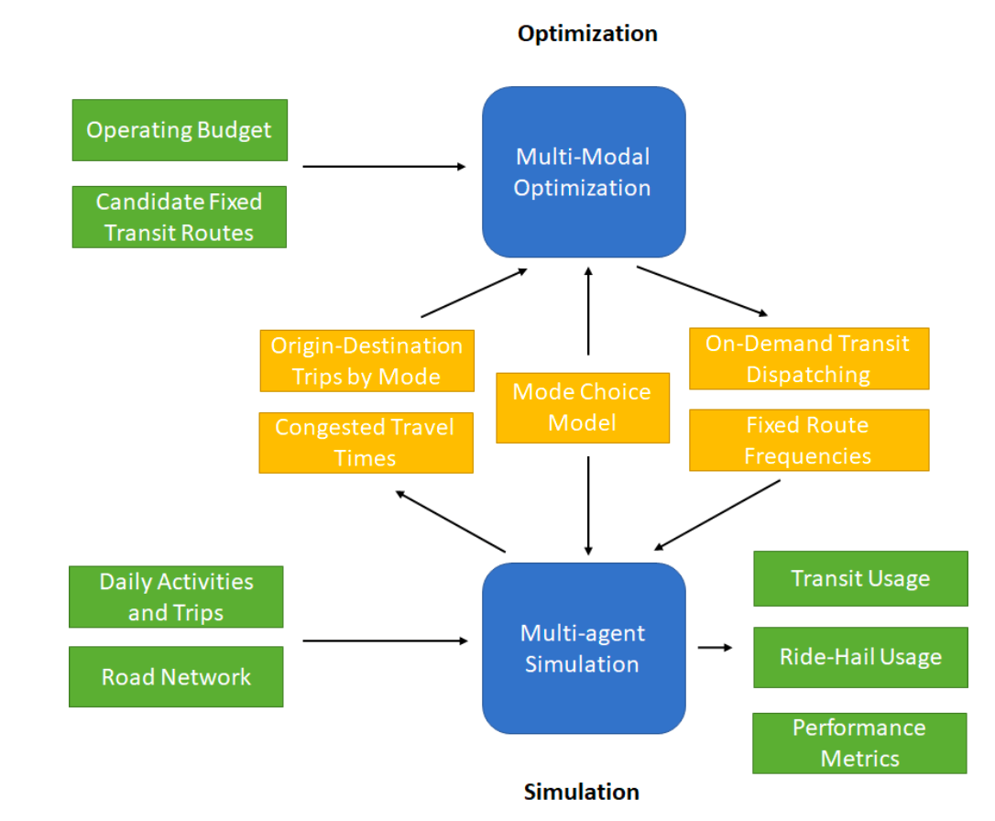
\includegraphics[width=0.75\linewidth]{pics/mmos} 

}

\caption{Overview of the T-SCORE MMOS tract process.}\label{fig:mmos}
\end{figure}

Creating consistency between the mode choice models for all the moving parts of the MMOS tract was crucial to creating a reliable product. We hypothesized that a consistent mode choice model would minimize error in predicting the effectiveness of inserting on-demand transit vehicles into any given region. For example, an inconsistency between one mode choice model over another could result in an inaccurate prediction of needing 100 vehicles in an area. In reality though, that area truly only needs 25 on-demand transit vehicles. Therefore, in an effort to minimize error in predicting on-demand transit vehicle use, a consistent mode choice model was desired. With that consistent mode choice model, answering the question on whether or not on-demand transit vehicles can help solve the first-mile/last-mile transit problem becomes possible.

\hypertarget{purpose-of-research}{%
\section{Purpose of Research}\label{purpose-of-research}}

This research, as inspired by the mode choice model within the MMOS tract of the T-SCORE project, includes one primary objective. That objective is to understand the effects of a consistent mode choice model between an activity-based model and a microsimulation tool. Along with understanding the effects of a consistent mode choice model, this research also aims to understand the effects of different types of mode choice utility parameters. Specifically the effects of predicting mode choice between path, person, and location type variables are explored. In addition, the effects of a consistent mode choice on subtour trip mode choice selection are analyzed. Overall, if consistent mode choice models were to better predict mode choice, we would make better predictions on how to implement new transportation strategies. Particularly, we would better understand how to implement on-demand transit vehicles in certain areas as to help solve the first-mile/last-mile transit problem.

Two important software were used to carry out the research objective. ActivitySim, an open-source advanced activity-based travel model, was used to create daily activity patterns (DAPs) for agents in the Salt Lake City, Utah region (ActivitySim 2021). BEAM, an agent-based microsimulation tool, was used to model the DAPs of the agents (BEAM 2022). BEAM has the capability to accomplish within-day planning where agents are able to dynamically respond to new transportation services. This project's main objective was carried out by changing BEAM's default mode choice model to more closely align with that of ActivitySim's. The details behind each software and their mode choice model will be discussed further on in the thesis.

\hypertarget{outline-of-research}{%
\section{Outline of Research}\label{outline-of-research}}

Chapter 1 introduces the objectives and motives behind the research. This chapter also give the outline to the thesis. In Chapter 2 an extensive literature review on mode choice modeling is conducted. Chapter 2 begins by explaining mode choice in the four step model as well as giving a brief history of mode choice in discrete choice modeling. Afterwards, the broad range of mode choice models used in activity-based models are explained. Then, the mode choice models of ActivitySim, MATSim, and BEAM are described in detail. Finally, the research gap is provided explaining the need for understanding the importance of mode choice consistency.

Chapter 3 describes the methods that were taken in order to answer the research questions presented. First, how the test scenario was created is explained. This also involves understanding the set up of ActivitySim and BEAM for the Salt Lake City, Utah region. After explaining the setup process, the methods toward creating an improved mode choice model in BEAM are described. An explanation on data validation and calibration follows.

Chapter 4 describes the results of having a consistent mode choice model within the BEAM model. Specifically, this chapter explains three tests used to verify the effects of mode choice consistency. The first test compares total modal distributions. The second test aims to show the effects of different types of mode choice utility parameters. Finally, the third test shows the differences in subtour mode choice between the BEAM and ActivitySim models.

Chapter 5 has the purpose of reviewing the results and determining the effects of the research as a whole. It also describes what the next steps moving forward are as well as the limitations in this research. A conclusion is then given in Chapter 6 where the wider implications are explained and the first-mile/last-mile problem is restated.

\hypertarget{literature-review}{%
\chapter{Literature Review}\label{literature-review}}

\hypertarget{overview}{%
\section{Overview}\label{overview}}

Mode choice models are essential components in the transportation planning process. Key investment decisions along with other transportation decisions rely on the determination of individual mode choices within a population. Whether mode choice is estimated in a four step model, an activity-based model, or an agent based model, its level of significance remains the same.

\hypertarget{lit1}{%
\section{Mode Choice in the Four Step Model}\label{lit1}}

The four step model (FSM) has been the primary tool in person travel demand modeling since its development (McNally 2000). Although travel is theorized to be derived from activity participation, the FSM focuses on modeling with trip-based not activity-based travel methods. The methodology presented in the FSM is mostly universal. The FSM can be divided up into two stages. The first defining the traveler and land use characteristics and the second defining the demand on a transportation network and the travel characteristics (McNally 2000).

As its name suggests, the FSM includes four different steps: trip generation, trip distribution, mode choice, and route choice. In trip generation the magnitude of total trips is estimated and in trip distribution those trips are disbursed along different directions of travel. In mode and route choice, a multitude of variables are used to determine specifically how travel occurs.

Of the four steps in the FSM, mode choice in particular is a diverse, variable, and disaggregate step among different modeling applications. According to McNally (2000), mode choice is almost exclusively modeled on a disaggregate level within separate choice-based sampling. Choice probabilities are calculated on the individual trip level. McNally (2000) also mentions that with transit, carpooling vehicles, automobile tolls, and other new factors the mode choice algorithm can become extensive and difficult to determine. One common method used to estimate mode choice probabilities is a nested logit model (see Section \ref{lit3}). These mode choice models can reflect trip-maker characteristics as well as multiple performance variables (Ortuzar and G.Willumsen 1994; McNally 2000). Most applications of the FSM require multiple iterations of the mode choice and trip distribution steps in order to approximate formal convergence. Like with the nested logit model, discrete choice modeling has historically been the preferred method in estimating mode choice in the FSM as well as in other modeling applications.

\hypertarget{lit2}{%
\section{A Brief History of Mode Choice in Discrete Choice Models}\label{lit2}}

Various choice modeling systems have been used to accurately determine mode choices. The beginning of such analyses started with the developments of McFadden et al. (1973), who outlined a general procedure for modeling population choice behavior from distributions of individual decision rules. Before then, discrete choices were simply modeled using a random utility model (RUM) framework. The interpretation assumed that each individual carried their own utility function distribution and selected one randomly; according to Manski (2001), McFadden reinterpreted the random assignment of the utility functions across the population itself rather than the individual. This yielded an entirely new view of discrete choice modeling, and a more general version of the multinomial logit model (MNL) was introduced. This new MNL model, also called the conditional logit analysis, was the beginning of modern mode choice analysis. Goulias, Davis, and Bhat (2020) describe that McFadden's MNL model, the nested logit model, and the multinomial probit model (MNP) were the main engines in mode choice and most discrete choice analyses up through the 1990s.

Although the developments of McFadden are still in effect today, mode choice analysis has evolved greatly in the last few decades. Goulias, Davis, and Bhat (2020) explain that up through 2010, mixed multinomial logit (MMNL) models and multiple discrete-continuous (MDC) choice models were the main models in practice. In addition, Bhat (1995) estimated a disaggregate mode choice model to explain how new and updated services affected ridership and mode choice on intercity travel. His heteroscedastic extreme value model overcame the independence of irrelevant alternatives (IIA) property and allowed more flexibility among the alternatives than the nested logit model. Ben-Akiva, Mcfadden, et al. (2002) developed a hybrid choice model (HCM) that went beyond the standard RUM as it included latent variables, latent classes, and a flexible error structure. It implemented multiple facets of discrete choice modeling and more accurately represented the behaviors of the individuals. Pinjari et al. (2007) used a simultaneous mixed logit model to understand how commuters' mode choice is affected by the surrounding build environment.

According to Goulias, Davis, and Bhat (2020), from 2010 to 2015 joint models of data with mixed dependent variables arrived. Vij, Carrel, and Walker (2013), for example, used a behavioral mixtures model, composed of a latent class choice model (LCCM) and a continuous logit mixture model, to extrapolate unobserved modality styles and their effects on travel decisions. Paulssen et al. (2014) focused on improving the integrated choice and latent variable (ICLV) model of McFadden (1986) and Ben-Akiva, Walker, et al. (2002) by including a value system among the individuals. Overall, the general advancement within mode choice and discrete choice modeling is comprehensive across recent years. Similarly, the variability among mode choice analysis can specifically be seen within activity-based modeling.

\hypertarget{lit3}{%
\section{An Extensive Look into Mode Choice in Activity-Based Models}\label{lit3}}

A significant part of activity-based modeling is the mode choice decision within the model. Bhat and Koppelman (1999) stated that originally travel demand models used individual trips as the primary unit of analysis. In recent years though, there has been a shift toward activity-based travel demand modeling. According to Eluru et al. (2010), this shift has occurred due to improved understanding of activity-based travel, global climate concerns, and advances in microsimulation techniques. With this shift to activity-based travel modeling, FSMs have evolved immensely, and especially within the last decade (Hasnine and Nurul Habib 2021). A major maturing in activity scheduling, activity duration, activity generation, and location choice has occurred and resulted in advanced activity-based modeling. Although these components have evolved significantly, the mode choice decision has remained relatively simple and constant.

In general, the two types of mode choice models commonly applied in travel demand modeling are trip-based and tour-based models. Trip-based mode choice models select modes based on the characteristics of individual trips, independent of other existing trips. A tour is defined as a chain of trips that end in the same location as they start (John L. Bowman et al. 1999). Tour-based models are based on the characteristics of the trips' overarching tour, meaning trip modes are not independently calculated. Most activity-based models commonly implement the tour-based mode choice structure (Hasnine and Nurul Habib 2021).

The most common use of the tour-based mode choice model is the ``simplified tour-based'' mode choice model. The simplified tour-based model has been used in a variety of studies (Arentze and Timmermans 2000; J. L. Bowman and Ben-Akiva 2001; Ram M. Pendyala et al. 1997). This simplified model hinges on trip-based mode choice where a single mode is used to define the entire tour opposed to a string of possible mode option combinations. For example, a simplified tour-based mode choice would define the tour-mode as ``public transit'' whereas a true tour-based model would define the tour-mode as ``public transit - ride hail - public transit''. Simplified tour-based models overlooks mobility attributes as well as the dynamics that exist between trips on a tour (Hasnine and Nurul Habib 2021).

There have been many attempts during the last few decades to include trip and tour based mode choice models into activity-based models. As a way to better understand the diversity that exists with tour-based mode choice in activity-based models, Hasnine and Nurul Habib (2021) conducted research on a variety of activity-based models from the years 1995 to 2020 and found that seven specific mode choice analyses have been used. All seven techniques are framed about the tour-based methodology further reinforcing the knowledge that ``the tour-based approach is the most relevant to the activity-based modelling framework'' (Hasnine and Nurul Habib 2021). These seven categories are further discussed in the following subsections.

\hypertarget{lit31}{%
\subsection{Simplified main tour model}\label{lit31}}

The simplified main tour model is another name for the simplified tour-based model previously discussed and implemented in most activity-based modeling applications (Arentze and Timmermans 2000; J. L. Bowman and Ben-Akiva 2001; Ram M. Pendyala et al. 1997). In the A Learning-Based Transportation Oriented Simulation System (ALBATROSS) developed by Arentze and Timmermans (2000), for example, when individuals had a work activity in their daily plan, a transport mode was determined for the work travel purpose. A singular tour mode value was selected and given to that individual. In cases where households had less cars than people, a car tour mode assigned to one individual in a household prevented a car mode being given to another individual in that same household. The simplified main tour model keeps track of car ownership and availability in a logical way. The ALBATROSS system selected the tour mode based on a subset of rules and decision trees programmed into the model. This means that the ALBATROSS system only allowed each trip within a tour to have the same mode as the tour mode (Arentze and Timmermans 2000).

Since a singular mode value is assigned to the tour in the simplified main tour model method, no flexibility exists for trip mode selection. Once a tour mode is determined, that same mode is held constant for each trip within that tour. Although not entirely realistic, many modelers prefer this method as it is a computationally easier task than a tour-based mode choice that permits trip modes to be different than their overarching tour mode. Realistically, however, individuals often vary their modes on different trips within a tour. For example, those who walk or bike or drive to transit are unable to do so in a simplified main tour model. Using the simplified main tour mode choice model may be popular and computationally simple, but it is not dynamic or realistic in representing travel behavior (Hasnine and Nurul Habib 2021).

\hypertarget{lit32}{%
\subsection{Two-tier nested logit model}\label{lit32}}

The two-tier nested logit model first completes an upper-level location choice followed by a lower-level mode choice which corresponds to the destination's location. One example of this approach being implemented in the literature is the Florida Activity Mobility Simulator (FAMOS) model (Ram M. Pendyala et al. 2005). The FAMOS model uses both the Household Attributes Generation System and the Prism-Constrained Activity-Travel Simulator in order to model activity patterns. The sub models within FAMOS include an activity-type choice, a joint destination and mode choice, and an activity duration choice. Additionally, FAMOS mode choice model first determines the destination location, and then selects a mode dependent on the destination location. Although it uses a two-tier nested logit model, Hasnine and Nurul Habib (2021) states that a tour-based mode choice is not ``explicitly identified'' in the FAMOS model. At its development, FAMOS gave promising results in the effectiveness of an activity-based modeling system (Ram M. Pendyala et al. 2005). It did not however include an extensive mode choice model.

\hypertarget{lit33}{%
\subsection{Simplified main tour mode and conditional trip-level mode}\label{lit33}}

The simplified main tour mode and conditional trip-level mode choice model has two parts. First a tour mode is estimated. Then, conditional on the estimated tour mode and attributes of the activity, trip modes are estimated. One example of a model that uses this structure is called DaySim (John L. Bowman, Bradley, and Gibbs 2006). DaySim follows the same activity scheduling approach developed by J. L. Bowman and Ben-Akiva (2001). The DaySim model is a microsimulation model that works off of four levels: long term person/household decisions, single day activity patterns, tour-level decisions, and trip-level decisions. The mode choice structure within DaySim involves a series of logsums and approximated logsums in order to econometrically estimate individual mode choice. More specifically, first a logsum is used to determine an overarching tour mode. This mode is used for all trip modes under that tour for the first steps within the model (John L. Bowman, Bradley, and Gibbs 2006). Later, however, trip modes are updated individually based on the tour mode value, origin and destination locations, and start times. The mode choice approach in DaySim is effective in that it relies heavily on fundamental econometric theories and allows trip modes to vary from tour modes (Hasnine and Nurul Habib 2021).

Other examples in the literature also use the simplified main tour mode and conditional trip-level mode choice structure, however only the details relating to ActivitySim's mode choice structure will be discussed further (see Section \ref{lit4})

\hypertarget{lit34}{%
\subsection{An activity-based model with exogenous mode choice}\label{lit34}}

The idea behind this mode choice model is that the mode choice decision is not estimated within the activity-based model, but estimated outside of it. One example of an activity-based model with the mode choice decision estimated exogenously is the comprehensive utility-based system of activity-travel scheduling options modelling (CUSTOM). The research done by Nurul Habib (2017) using the CUSTOM system assumed an exogenous mode choice. This meant that the mode specific travel time used to estimate travel behavior was an explanatory variable in the model. Nurul Habib (2017) mentions that the exogenous mode choice was a limitation in their research and further research is needed to specify how to seamlessly align the exogenous mode choice into the CUSTOM structure. Hasnine and Nurul Habib (2021) also mentions that a limitation to this mode choice model is that the mode is not modeled endogenously with other activity attributes.

\hypertarget{lit35}{%
\subsection{Simulation-based tour-based mode choice}\label{lit35}}

The simulation-based tour-based mode choice model is a simulation-based approach to estimating modes when large sets of modal alternatives are present. An example of this approach in the literature is a model used by Miller, Roorda, and Carrasco (2005) called the Travel/Activity Scheduler for Household Agents (TASHA). TASHA is both agent-based and activity-based where decisions are modeled using a random utility framework. In addition, TASHA is both chain-based and trip-based meaning that individual trips have individual modes chosen, but tour modes are constructed in a chain-based manner. Utility functions are used to calculate the utility of both individual trip modes as well as chains of modes used in the tour-based mode choice model. TASHA adopts a probit modeling structure in order to determine probabilities of modal alternatives (Miller, Roorda, and Carrasco 2005; Hasnine and Nurul Habib 2021). This simulation approach is computationally heavy but is effective in providing unique trip modes based on chain-based tour modes.

Another example of a simulation-based mode choice model is presented by Eluru et al. (2010). Eluru et al. (2010) developed a joint multiple discrete continuous extreme value (MDCEV) framework to model the individual's choices across five dimensions: activity type, time of day, mode, destination, and time use. The MDCEV framework aimed to model activity travel choices simultaneously.

\hypertarget{lit36}{%
\subsection{Combinatorial tour-based mode choice}\label{lit36}}

The combinatorial tour-based mode choice model simulates all combinations of modes within any given tour. A utility value is then calculated for each combination of trip modes and a logit model is used to determine which combination any given agent will select. This method is computationally heavy, but allows the possibility for any combination of modes to exist (Hasnine and Nurul Habib 2021). An example of this model being used in practice is the research conducted by Vovsha et al. (2017).

\hypertarget{lit37}{%
\subsection{Dynamic tour-based mode choice}\label{lit37}}

Dynamic tour-based mode choice models are programmed with dynamic discrete choice modeling. The central idea is to model sequential discrete choices in order to determine current and future outcomes. Saleem, Västberg, and Karlström (2018) provides an example of implementing a dynamic tour-based mode choice model in the random utility based travel model named SCAPER. SCAPER makes decisions sequentially in time, based on random utility theory. MATSim also implements the SCAPER model by generating activity schedules, activity duration, activity locations, and mode choices. MATSim iteratively updates the mode choice based on the best modal option available, and continues to iteratively update mode choice until schotastic equilibrium is reached (Hasnine and Nurul Habib 2021). More intimate details inside the MATSim mode choice model will be discussed later on in Section \ref{lit5}.

Overall, the seven categories of mode choice presented by Hasnine and Nurul Habib (2021) gives a good overview on the details behind existing mode choice structures within activity-based models. It is shown that although trip-based models have been used, tour-based mode choice models are the prominent form of mode choice modeling in activity-based models. ActivitySim is the activity-based model used in this research, and so the details of its mode choice structure will be analyzed more closely in Section \ref{lit4}.

\hypertarget{lit4}{%
\section{The Mode Choice Models used in ActivitySim}\label{lit4}}

The activity-based model used in this research to generate activity plans is ActivitySim. ActivitySim is an activity simulator used to generate plans for millions of agents each with their own demographic attributes (Gali et al. 2008). Instead of independently modeling each trip, ActivitySim simulates each individual and their daily travel diaries and schedules. Since ActivitySim forecasts travel based on a disaggregate population, more realistic travel estimates are generated than can be generated by forecasting travel using aggregate trips. Long term decisions are made first, and then shorter term decisions are calculated based on the long term decisions ({``ActivitySim: An Advanced Activity-Based Travel Demand Model Built by and for Users''} 2021). Overall, ActivitySim is an advanced activity-based model that is cost effective, user friendly, and efficient at forecasting travel behavior.

As discussed in Section \ref{lit33}, ActivitySim adopts a simplified main tour mode model and a conditional trip-level mode model for its mode choice framework. The specifics of this dual level mode choice is described further in its application by MTC (2012).
The mode choice model in ActivitySim is multifaceted between tours, trips, and purpose. In other words, there is a mode choice model that determines the \emph{primary} mode for each tour and a separate mode choice model that determines the mode for each trip within each tour (MTC 2012). The tour choice is the upper-level choice whereas the trip mode choice is the lower-level choice that is conditional upon the upper-level choice. Two levels of mode choice is more advanced than the simplified main tour mode choice model.

This overarching mode choice structure exists separately for each purpose. This means that since there are ten purposes specified in ActivitySim, there are ten tour mode choice models and ten trip mode choice models.

Multiple travel statistics are calculated at the trip and the tour level. At the tour level the tour modes, stop frequencies, and stop locations are estimated. Then, at the trip level the departure times, trip modes, parking for automobiles, and vehicle assignments are determined ({``ActivitySim: An Advanced Activity-Based Travel Demand Model Built by and for Users''} 2021).

\hypertarget{lit41}{%
\subsection{ActivitySim's Tour Mode Choice Model}\label{lit41}}

The tour mode choice model assigns the primary mode that is used to get from origin to destination. This level accounts for variables that affect the entire tour. The tour mode decision also affects the alternative values that are available for each trip. The specific details that determine which mode is used for each tour have to do with whether the tour is done by private car or by public transit, walking, or biking; whether there is carpooling available; and whether the transit mode is accessible by foot or by car (MTC 2012).

The specific choice model used to determine the overarching tour mode is a nested logit model. It separates similar modes into differing bins as to ``more accurately model the cross-elasticities between the alternatives'' (MTC 2012). Figure \ref{fig:fig1} shows all 18 modes within ActivitySim and how they fit within the nested logit structure.

\begin{figure}

{\centering 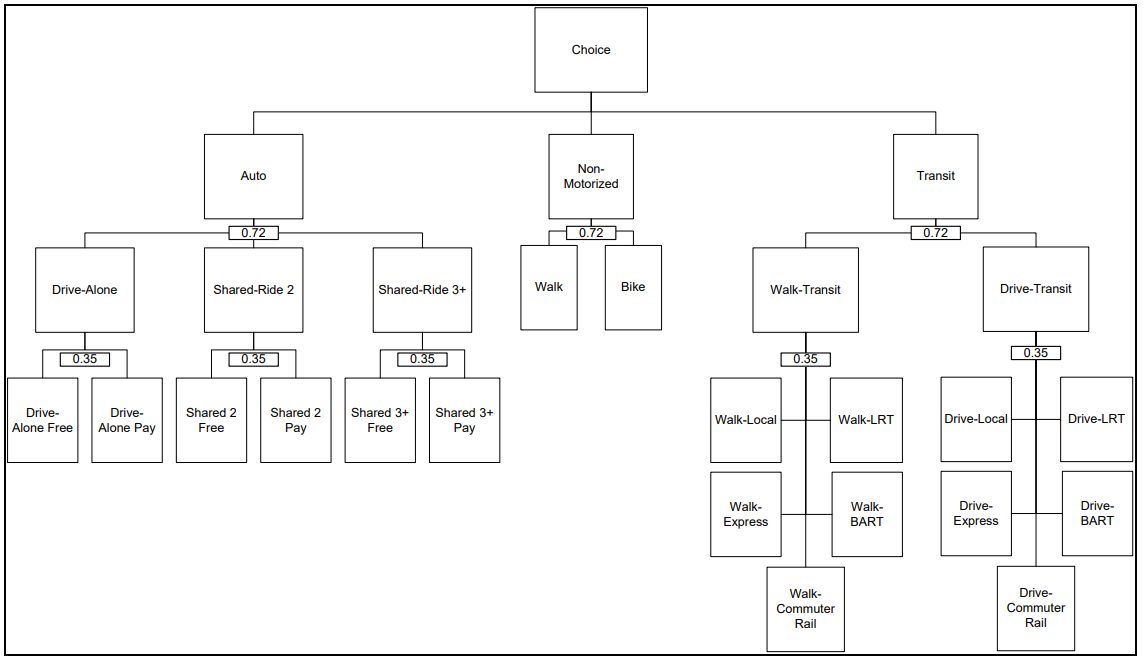
\includegraphics[width=1\linewidth]{pics/tour_nest} 

}

\caption{Tour Mode Choice Nested Logit Model (MTC 2012).}\label{fig:fig1}
\end{figure}

The first division of modes is describes whether it is an automobile, a non-motorized vehicle, or a transit type. In a broad sense, the second level of nesting for automobile and non-motorized has to do with vehicle occupancy. If it is an automobile, three secondary bins exist: drive-alone, shared-ride with two people, and shared-ride with three or more people. Then, in the third level of nesting, two bins exist having to do with if the mode is free or not. On the other hand, the non-motorized section is only divided up into the walk or bike mode, with no options on the third level. The transit nest is divided into walk-transit and drive transit on the secondary level. There are then five more bins within each one of those transit options having to do with which specific transit type is involved, like LRT, express, etc. The logsum coeffiecient for the first nest is 0.72 and for the second nest 0.35 (MTC 2012).

The utility functions for each mode are shown in Section \ref{lit411}. The primary variables in the utility functions are in-vehicle time, other travel times, cost, characteristics of the destination zone, demographics, and auto ownership of the household. Each mode has different parameter values for each one of the variables, for each tour purpose value.

\hypertarget{lit411}{%
\subsection{ActivitySim's Tour Mode Choice Utility Functions}\label{lit411}}

The utility functions for the auto, nonmotorized, and transit tour modes are presented in this section.

All \(\beta\) and \(ASC\) values are meant to represent parameter values. All other variables are dependent on other things, like time for example. (The utility equations are deduced from information from MTC (2012)).

\textbf{Auto}

\(V_{DriveAlone} = IVTT(\beta_{IVTT}) + ASC_{DA1619}\)

\(V_{Shared2} = IVTT(\beta_{IVTT}) + OVTT_w(\beta_{OVTT_w}) + ASC_{DA16P} + ASC_{HHS} + ASC_{ITC} + ASC_{JTC}\)

\(V_{Shared3P} = IVTT(\beta_{IVTT}) + OVTT_w(\beta_{OVTT_w}) + ASC_{DA16P} + ASC_{HHS} + ASC_{ITC} + ASC_{JTC}\)

\begin{itemize}
\tightlist
\item
  \(IVTT\) is the in-vehicle travel time (min),
\item
  \(OVTT_w\) is the initial wait time (min); \(\beta_{OVTT_w}\) is different depending on if \(OVTT_w\) is above or below 10 minutes,
\item
  \(ASC_{DA1619}\) is a demographic variable for individuals between 16-19 years old,
\item
  \(ASC_{DA16P}\) is a demographic variable for individuals 16 years old or older,
\item
  \(ASC_{HH}\) is a demographic variable for household size; different depending on size,
\item
  \(ASC_{ITC}\) is an individual tour constant; different depending on ratio of number of cars to number of workers, and
\item
  \(ASC_{JTC}\) is a joint tour constant; different depending on ratio of number of cars to number of workers
\end{itemize}

\textbf{NonMotorized}

\(V_{Walk} = DIS(\beta_{DIS}) + ZTI(\beta_{ZTI}) + ZDI_d(\beta_{ZDI_d}) + ZDI_o(\beta_{ZDI_o}) + ASC_{ITC} + ASC_{JTC}\)

\(V_{Bike} = DIS(\beta_{DIS}) + ZTI(\beta_{ZTI}) + ZDI_d(\beta_{ZDI_d}) + ZDI_o(\beta_{ZDI_o}) + ASC_{ITC} + ASC_{JTC}\)

\begin{itemize}
\tightlist
\item
  \(DIS\) is the distance travled (miles); \(\beta_{DIS}\) is different depending on if \(DIS\) is above or below 1.5 miles for walk and 6 miles for bike,
\item
  \(ZTI\) is the zonal topography index at the destination,
\item
  \(ZDI_d\) is the zonal density index at the destination,
\item
  \(ZDI_o\) is the zonal density index at the origin,
\item
  \(ASC_{ITC}\) is an individual tour constant; different depending on ratio of number of cars to number of workers, and
\item
  \(ASC_{JTC}\) is a joint tour constant; different depending on ratio of number of cars to number of workers
\end{itemize}

\textbf{Transit}

\(V_{WalkTransit} = IVTT(\beta_{IVTT}) + [OVTT_w(\beta_{OVTT_w}) + OVTT_t(\beta_{OVTT_t}) + ASC_{OVTT_d} + ASC_{OVTT_o}] \\ \qquad + T(\beta_T) + ZTI(\beta_{ZTI}) + ZDI_d(\beta_{ZDI_d}) + ZDI_o(\beta_{ZDI_o}) + ASC_{T10} + ASC_{CBD} + ASC_{ITC} \\ \qquad + ASC_{JTC} + ASC_{TLH}\)

\(V_{DriveTransit} = IVTT(\beta_{IVTT}) + [OVTT_w(\beta_{OVTT_w}) + OVTT_t(\beta_{OVTT_t}) + OVTT_{dr}(\beta_{OVTT_{dr}})] \\ \qquad + T(\beta_T) + ZTI(\beta_{ZTI}) + ZDI_d(\beta_{ZDI_d}) +DIS_{15}(\beta_{DIS_{15}})+ ASC_{T10} + ASC_{CBD} + ASC_{ITC} \\ \qquad + ASC_{JTC} + ASC_{TLH}\)

\begin{itemize}
\tightlist
\item
  \(IVTT\) is the in-vehicle travel time (min); \(\beta_{IVTT}\) is different depending on which transit mode is selected,
\item
  \(OVTT_w\) is the initial wait time (min); \(\beta_{OVTT_w}\) is different depending on if \(OVTT_w\) is above or below 10 minutes,
\item
  \(OVTT_{dr}\) is the drive to transit time (min),
\item
  \(OVTT_t\) is the transfer wait time travel time (min),\\
\item
  \(ASC_{OVTT_d}\) is the destination walk time constant; different depending on short or long walk to destination,
\item
  \(ASC_{OVTT_o}\) is the origin walk time constant; different depending on short or long walk from origin,
\item
  \(T\) is the number of transfers,
\item
  \(ZTI\) is the zonal topography index at the destination,
\item
  \(ZDI_d\) is the zonal density index at the destination,
\item
  \(ZDI_o\) is the zonal density index at the origin,
\item
  \(DIS_{15}\) is the number of miles less than 15,
\item
  \(ASC_{T10}\) is a demographic variable for individuals under 10 years old,
\item
  \(ASC_{CBD}\) is a constant used if the destination is in CBD for area types 0 and 1,
\item
  \(ASC_{ITC}\) is an individual tour constant; different depending on ratio of number of cars to number of workers,
\item
  \(ASC_{JTC}\) is a joint tour constant; different depending on ratio of number of cars to number of workers, and
\item
  \(ASC_{TLH}\) is the transit line-hail mode constant; different depending on which transit mode is selected.
\end{itemize}

\hypertarget{lit42}{%
\subsection{ActivitySim's Trip Mode Choice Model}\label{lit42}}

The trip mode choice model assigns a specific mode to each trip on a given tour. It is similar to the tour mode choice model, except only certain trips are allowed depending on the tour mode. Figure \ref{fig:fig2} displays a detailed explanation of which trip modes are allowed according to the tour mode that was selected in the tour mode choice.

\begin{figure}

{\centering 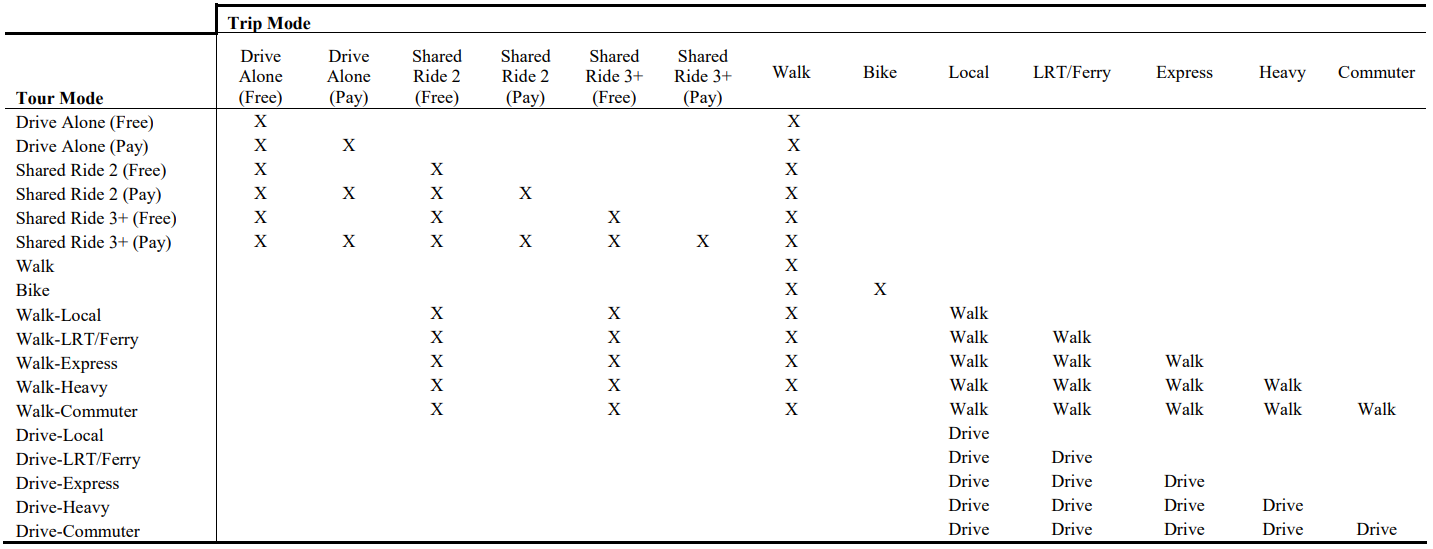
\includegraphics[width=1\linewidth]{pics/trip_allow} 

}

\caption{Trip Mode Availability based on Tour Mode (MTC 2012).}\label{fig:fig2}
\end{figure}

The rules that define the correspondence between trips and tours are defined as the following: (MTC 2012)

\begin{enumerate}
\def\labelenumi{\arabic{enumi}.}
\item
  Pay trip modes are only allowed under pay tour modes. For example, Shared Ride 2 (Pay) is only an available trip under the tour mode Shared Ride 2 (Pay).
\item
  The auto occupancy for the tour mode is determined by the maximum auto occupancy among all the auto trips within the tour. Therefore, the tour mode's auto occupancy is the trip with the largest auto occupancy within the tour.
\item
  Transit tours do allow auto-shared (carpooling) trips for particular legs. For example, if someone takes an auto-shared trip to work, the mode choice structures allows the individual to take transit back home.
\item
  The walk mode is an allowed mode for any given trip, no matter the tour.
\item
  ``The availability of transit line-haul submodes on transit tours depends on the skimming and tour mode choice hierarchy'' (MTC 2012). Albeit a low probability, free shared-ride trip modes are allowed in walk-transit tours. Paid shared-ride trip modes are not allowed, however, on transit tours because no evidence promotes this mode selection.
\end{enumerate}

The utility function equations used for the trip mode choice model are shown in Section \ref{lit421}. These parameters are very similar to the ones used in the tour mode choice model. In most cases, the in-vehicle times for coefficients in the trip mode choice are identical with the in-vehicle times in the tour mode choice. For coefficients of variables that apply in the trip mode choice to multiple legs, but only apply once in the tour mode choice, the trip mode choice in-vehicle time is half that of the tour mode choice in-vehicle time.

The trip is determined using a nested logit model structure, just like the tour mode choice model. There is one for each tour purpose as well. Notice how it is based on \emph{tour} purpose and not each \emph{trip} purpose.

\hypertarget{lit421}{%
\subsection{ActivitySim's Trip Mode Choice Utility Functions}\label{lit421}}

The utility functions for the auto, nonmotorized, and transit trip modes are presented in this section. All \(\beta\) and \(ASC\) values are meant to represent parameter values. All other variables are dependent on other things, like time for example. (The utility equations are deduced from information from MTC (2012)).

\textbf{Auto}

\(V_{DriveAlone} = IVTT(\beta_{IVTT})\)

\(V_{Shared2} = IVTT(\beta_{IVTT}) + OVTT_w(\beta_{OVTT_w}) + ASC_{HHS} + ASC_{ITC}[TM_{S2}, TM_{S3P}, TM_T]\)

\(V_{Shared3P} = IVTT(\beta_{IVTT}) + OVTT_w(\beta_{OVTT_w}) + ASC_{HHS} + ASC_{ITC}[TM_{S3P}, TM_T]\)

\begin{itemize}
\tightlist
\item
  \(IVTT\) is the in-vehicle travel time (min),
\item
  \(OVTT_w\) is the initial wait time (min); \(\beta_{OVTT_w}\) is different depending on if \(OVTT_w\) is above or below 10 minutes,
\item
  \(ASC_{HH}\) is a demographic variable for household size; only used if the household size is 1,
\item
  \(ASC_{ITC}\) is an individual tour constant,
\item
  \(TM_{S2}\) is a tour mode indicator for the Shared2 mode (1 if the tour mode is Shared2 and 0 if not),
\item
  \(TM_{S3P}\) is a tour mode indicator for the Shared3P mode(1 if the tour mode is Shared3P and 0 if not), and
\item
  \(TM_{T}\) is a tour mode indicator for a Transit mode(1 if the tour mode is Transit and 0 if not)
\end{itemize}

\textbf{NonMotorized}

\(V_{Walk} = DIS(\beta_{DIS}) + ZTI(\beta_{ZTI}) + ZDI_d(\beta_{ZDI_d}) + ZDI_o(\beta_{ZDI_o}) \\ \qquad+ ASC_{ITC}[TM_{DA}, TM_{S2}, TM_{S3P}, TM_{B}, TM_{T}]\)

\(V_{Bike} = DIS(\beta_{DIS}) + ZTI(\beta_{ZTI}) + ZDI_d(\beta_{ZDI_d}) + ZDI_o(\beta_{ZDI_o})\)

\begin{itemize}
\tightlist
\item
  \(DIS\) is the distance travled (miles); \(\beta_{DIS}\) is different depending on if \(DIS\) is above or below 1.5 miles for walk and 6 miles for bike,
\item
  \(ZTI\) is the zonal topography index at the destination,
\item
  \(ZDI_d\) is the zonal density index at the destination,
\item
  \(ZDI_o\) is the zonal density index at the origin,
\item
  \(ASC_{ITC}\) is an individual tour constant,
\item
  \(TM_{DA}\) is a tour mode indicator for the DriveAlone mode (1 if the tour mode is DriveAlone and 0 if not),
\item
  \(TM_{S2}\) is a tour mode indicator for the Shared2 mode (1 if the tour mode is Shared2 and 0 if not),
\item
  \(TM_{S3P}\) is a tour mode indicator for the Shared3P mode(1 if the tour mode is Shared3P and 0 if not), and
\item
  \(TM_{B}\) is a tour mode indicator for the Bike mode (1 if the tour mode is Bike and 0 if not), and
\item
  \(TM_{T}\) is a tour mode indicator for a Transit mode(1 if the tour mode is Transit and 0 if not)
\end{itemize}

\textbf{Transit}

\(V_{WalkTransit} = IVTT(\beta_{IVTT}) + [OVTT_w(\beta_{OVTT_w}) + OVTT_t(\beta_{OVTT_t}) + ASC_{OVTT_d} + ASC_{OVTT_o}] \\ \qquad + T(\beta_T) + ZTI(\beta_{ZTI}) + ZDI_d(\beta_{ZDI_d}) + ZDI_o(\beta_{ZDI_o}) + ASC_{ITC}[TM_T]\)

\(V_{DriveTransit} = IVTT(\beta_{IVTT}) + [OVTT_w(\beta_{OVTT_w}) + OVTT_t(\beta_{OVTT_t}) + OVTT_{dr}(\beta_{OVTT_{dr}})] \\ \qquad + T(\beta_T) + ZTI(\beta_{ZTI}) + ZDI_d(\beta_{ZDI_d}) + ASC_{ITC}[TM_T]\)

\begin{itemize}
\tightlist
\item
  \(IVTT\) is the in-vehicle travel time (min); \(\beta_{IVTT}\) is different depending on which transit mode is selected,
\item
  \(OVTT_w\) is the initial wait time (min); \(\beta_{OVTT_w}\) is different depending on if \(OVTT_w\) is above or below 10 minutes,
\item
  \(OVTT_{dr}\) is the drive to transit time (min),
\item
  \(OVTT_t\) is the transfer wait time travel time (min),\\
\item
  \(ASC_{OVTT_d}\) is the destination walk time constant; different depending on short or long walk to destination,
\item
  \(ASC_{OVTT_o}\) is the origin walk time constant; different depending on short or long walk from origin,
\item
  \(T\) is the number of transfers,
\item
  \(ZTI\) is the zonal topography index at the destination,
\item
  \(ZDI_d\) is the zonal density index at the destination,
\item
  \(ZDI_o\) is the zonal density index at the origin,
\item
  \(ASC_{ITC}\) is an individual tour constant; different depending which transit mode is selected, and
\item
  \(TM_{T}\) is a tour mode indicator for a Transit mode(1 if the tour mode is Transit and 0 if not)
\end{itemize}

\hypertarget{lit5}{%
\section{The Mode Choice Models used in Agent-based Models}\label{lit5}}

Thus far, an extensive review of mode choice in activity-based models as well as the tour and trip mode choice choice models in Activitysim has been conducted. It is clear that an overarching tour mode value is essential to mode choice trip estimation in activity-based models. In ActivitySim, a multitude of person, path, and location variables are also needed to estimate accurate mode choice decisions.

As a comparison, we will now review the mechanics of mode choice in agent-based models / microsimulation tools. In Section \ref{lit6} the mode choice model of the agent-based model MATSim is discussed. Then, in Section \ref{lit7} the mode choice model of the agent-based model BEAM is discussed. The BEAM microsimulation tool is the agent-based model used extensively this research.

\hypertarget{lit6}{%
\section{The Mode Choice Model used in MATSim}\label{lit6}}

Microsimulation is a modeling tool used to simulate individual vehicle movement across a network for the purpose of evaluating the traffic performance of the entire system. MATSim, as mentioned in Section @ref(lit3.7), is an example of a microsimulation tool used today and implements a unique mode choice model.

W Axhausen, Horni, and Nagel (2016) explains that mode choice in MATSim, along with time choice, destination choice, and route assignment, are chosen through an iterative cycle where every agent optimizes its daily activity pattern by picking the best option after each iteration. After multiple iterations, the optimal choice is determined. Specifically, it uses scoring functions (like the Charypar-Nagel utility function) to help determine the optimal choice for each iteration. Equation \eqref{eq:eq1} shows the basic form of the Charypar-Nagel Function used in MATSim (W Axhausen, Horni, and Nagel 2016).

\begin{equation} 
  S_{plan} = \sum_{q=0}^{N-1} S_{act,q} + \sum_{q=0}^{N-1} S_{trav,mode(q)}
  \label{eq:eq1}
\end{equation}

In the Charypar-Nagel utility function, \(S_{plan}\) represents the utility of a plan, \(S_{act,q}\) represents the sum of all the activity utilities, and \(S_{trav,mode(q)}\) represents the sum of all the travel ``(dis)utilities'' (W Axhausen, Horni, and Nagel 2016). In other words, the plan's utility is computed from adding the activity utilities and subtracting the mode and travel utilities.

During each iteration, a new plan for the agent is calculated, resulting in different travel and mode values selected. After each iteration, the plan with the best overall ``score'' or utility is selected probabilistically among the previous and current iteration utility plans. As discussed in Section \ref{lit37}, MATSim continues to iteratively update mode choice until schotastic equilibrium is reached (Hasnine and Nurul Habib 2021). This action of determining the best modal alternative over a simulation process means that the mode choice model is a mix of a simulation-based model (Section \ref{lit35}) and a dynamic tour-based model (Section \ref{lit37}).

MATSim's mode choice programming contrasts greatly from ActivitySim's mode choice model. Various efforts have been proposed to create a more advanced mode choice model system in MATSim. These efforts will be further explained in Section \ref{lit8}. First, Section \ref{lit7} explores the mode choice model of a different microsimulation tool named BEAM.

\hypertarget{lit7}{%
\section{The Mode Choice Model used in BEAM}\label{lit7}}

Another microsimulation tool, similar to MATSim, is BEAM. BEAM stands for Beahvior, Energy, Autonomy, and Mobility and is being developed at the Lawrence Berkeley National Laboratory. According to El Zarwi, Vij, and Walker (2017), BEAM's framework is designed to model and forecast the adoption and diffusion of new transportation services. Originally, BEAM implemented a Latent Class Choice Model (LCCM) as the mode choice structure to more accurately model early adopters, imitators, and non-adopters of the new transportation services. BEAM's user guide, however, explains that the LCCM model is not currently being used, and instead something similar to a nested multinomial logit model is in effect. The observed utility function for the multinomial logit model includes parameters relating to travel time, cost, and a constant term.

BEAM's mutlinomial logit model takes in certain parameters and inputs and uses them to probabilistically estimate the likely mode choice for each user in their respective situation. Mathematically, the observable utility equation for the simple multinomial logit model in BEAM is shown in Equation \eqref{eq:beammnl}.

\begin{equation}
  V_j = ASC_j + \beta_{cost}(cost) + \beta_{time}(time) + \beta_{xfer}(numtransfers) 
    \label{eq:beammnl}
\end{equation}

where

\begin{itemize}
\tightlist
\item
  \(j\) is the modal alternative,
\item
  \(V_j\) is the observable portion of the utility equation,
\item
  \(ASC_j\) is the alternative specific constant, and
\item
  \(\beta_{cost}\), \(\beta_{time}\), and \(\beta_{xfer}\) are generic coefficients for the cost, time, and number of transfer parameters.
\end{itemize}

All things considered, the observable utility equation for BEAM's multinomial logit model is pretty simple. There are only three \(\beta\) coefficients along with one alternative specific constant. Also, in BEAM, utility equations are specific to different mode options. For example, the utility for car, walk, bike, etc. will all be different. Yes Equation \eqref{eq:beammnl} shows the overarching utility equations, but the alternative specific constant differs between different modes.

A total of nine different modal alternatives are available in BEAM. Unlike ActivitySim, no tour-mode structure exists. BEAM's mode choice is designed on a trip-based system. Figure \ref{fig:fig-mode-compare} highlights how BEAM's trip-based mode choice works and summarizes the difference between ActivitySim's mode choice and BEAM's mode choice.

\begin{figure}

{\centering 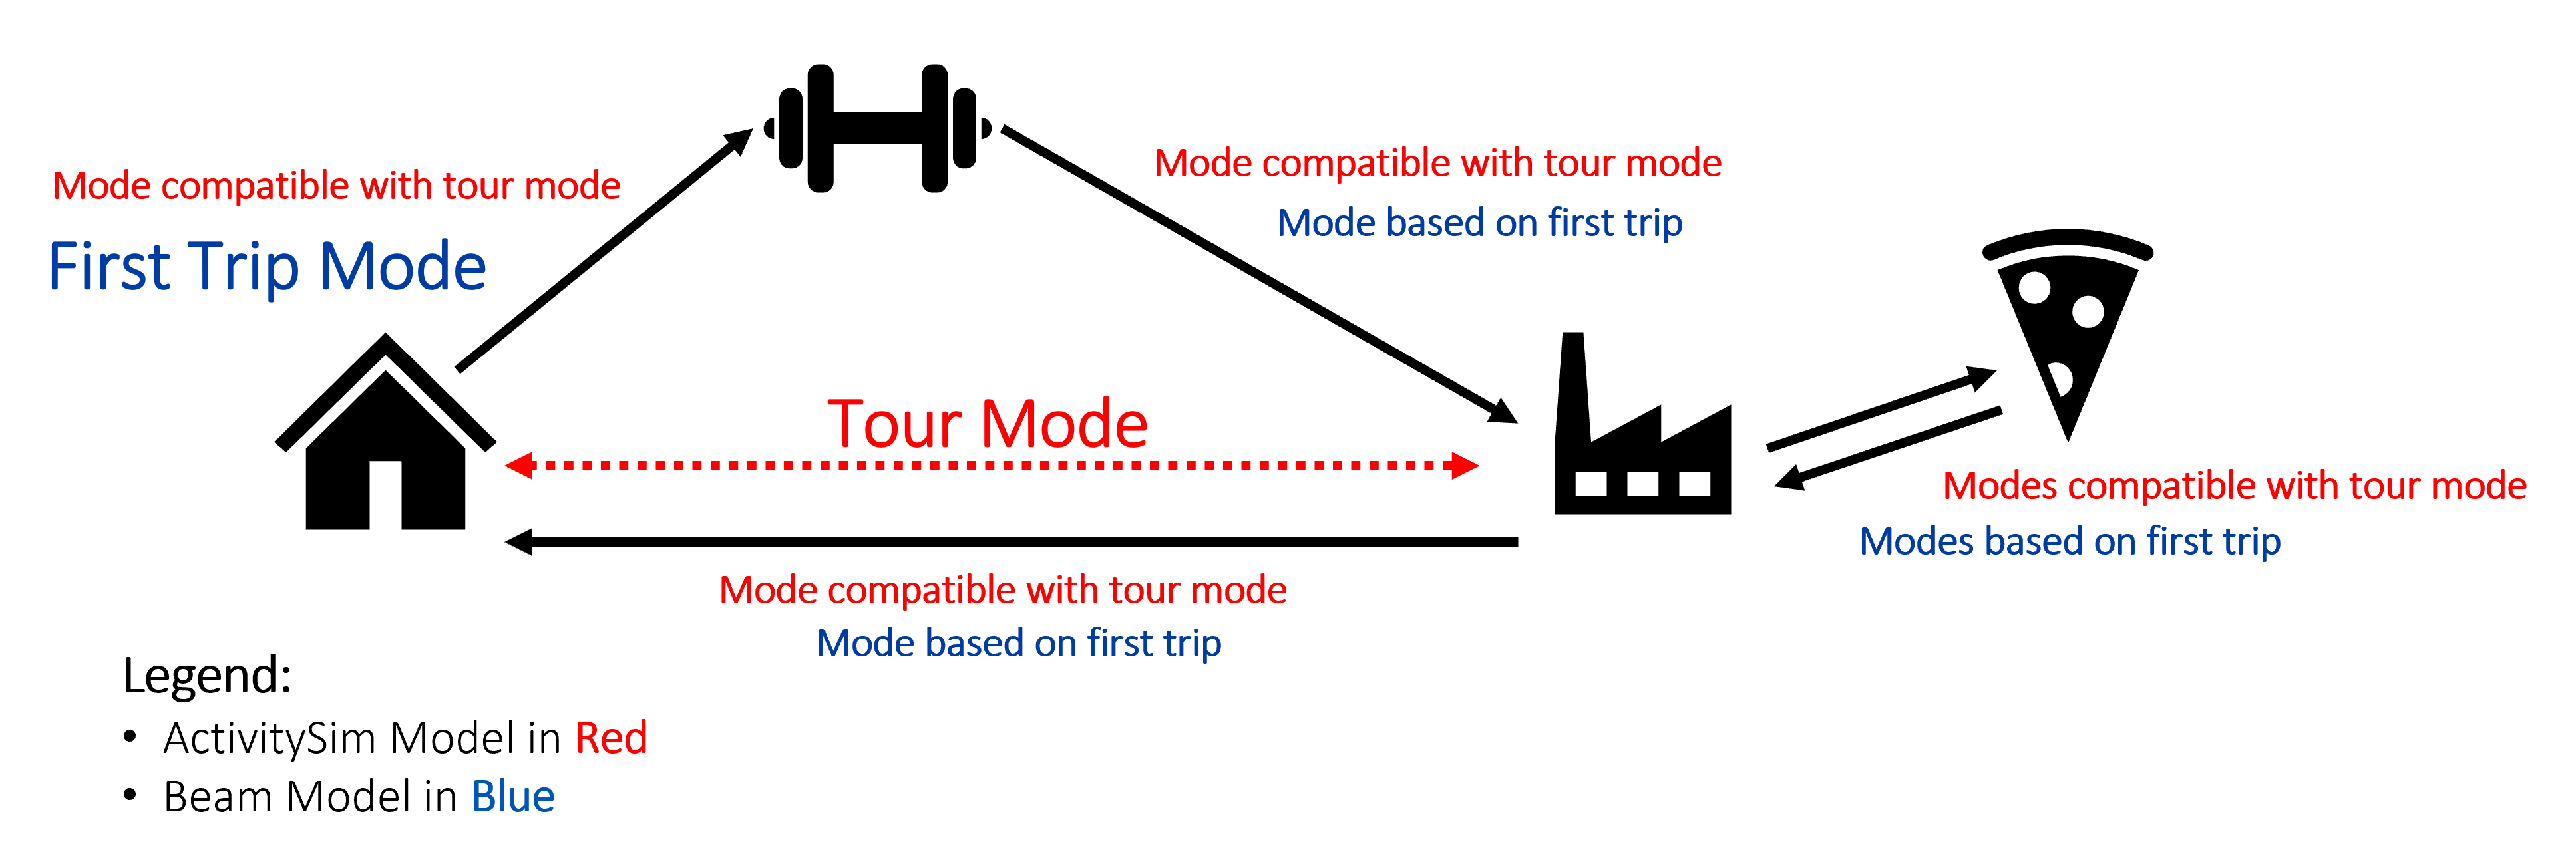
\includegraphics[width=1\linewidth]{pics/asim-beam-compare} 

}

\caption{Mode choice between ActivitySim and BEAM.}\label{fig:fig-mode-compare}
\end{figure}

ActivitySim provides mode choices off of the primary tour activity. For example, referring to in Figure \ref{fig:fig-mode-compare}, if a person wants to go to their work activity by train, ActivitySim knows that they can either walk or take transit to their gym activity. Contrastingly, BEAM bases mode choice on the first trip of the day. This means that BEAM will determine the optimal mode to go to the gym in, and then figure our how to get to work based on the first trip mode. In addition, ActivitySim knows that when a person leaves for lunch from their work activity, they will be returning back to their work activity after lunch. This means that the person is able to leave their car at work and possibly walk or take transit to and from their lunch activity. In BEAM though, if someone goes to lunch, they will most likely take their car as to not abandon their vehicle for the rest of their day. It is clear that BEAM's mode choice is less representative of how people actually transport themselves during the day. ActivitySim provides a better representation of mode choice. As a result, it is important to improve the mode choice model in BEAM (See Section \ref{lit8}).In this research we explore the importance of creating consistency between the mode choice models between BEAM and ActivitySim (See Section \ref{lit9}).

\hypertarget{lit8}{%
\section{Previous Attempts to Enhance Mode Choice in Agent-based Models}\label{lit8}}

In recent years, suggestions have been made on how to improve MATSim's mode choice structure. Axhausen, Balmer, and Ciari (2008) proposed introducing discrete choice, in the form of a multinomial logit model on the subtour level of mode choice. Currently, MATSim's mode choice is performed at the tour level, meaning subtour mode choice is limited. This new introduction would allow variation in mode on all subtours. Similarly, Hörl, Balac, and Axhausen (2018) proposed updating upon a subtour mode choice model to eliminate heavily randomized processes and to increase the use of realistic subtour modal options.

In addition to improving the subtour mode choice strategy within MATSim, Hörl, Balac, and Axhausen (2018) also proposed introducing a chain-based modal selection model, similar to the type of model discussed in Section \ref{lit36}. Hörl, Balac, and Axhausen (2018) describes this chain-based model with, ``If one iterates over all possible combinations of modes on these trips, one arrives at a set of available mode chains C of size \(M^{N}\), where \(M\) is the number of possible modes and \(N\) is the number of trips.'' The resulting set of feasible chains \(C_f \in C\) could look as follows:

\begin{equation} 
  C_f = \{(car,car,car),(transit,transit,transit),(transit,walk,transit),...\}
  \label{eq:eq2}
\end{equation}

Equation \eqref{eq:eq2} provides a great example of all the chain-based modal alternatives that would exist in the choice set. In order to model the chain selection, Hörl, Balac, and Axhausen (2018) suggest incorporating ``an out-of-the-box discrete mode choice model into MATSim''. They propose that this discrete choice model would involve two sampling approaches. The first approach involves calculating the total utility value for the chain-based modes and the other would be based on individual trip probabilities. In order to calculate the utility however, various variables like travel time and travel costs would be involved. The downside to this model would be that analyzing the chain-based modes and calculating individual utilities would cause significant computational overhead compared to MATSim's default mode choice model.

In the work done by Hörl, Balać, and Axhausen (2019), a discrete choice model is actually inserted into MATSim and tested using a case study of the city of Zurich. In this model, both a trip based and a tour based mode choice model are used. The tour based model is identical to the chain-based model described in the work done by Hörl, Balac, and Axhausen (2018). A multinomial logit model is used to probabilistically select between the utility values of each modal alternative. With the introduction of discrete choice and chain-based tour mode choice into MATSim, Hörl, Balać, and Axhausen (2019) states that there is better convergence behavior. Since mode choice is not done at random and no irrational modal decisions are being made, this newer model arrives at convergence with fewer iterations. However, since more explanatory variables are needed to estimate mode choice, extensive calibration is required in order to ensure the mode choice model performs in an unbiased manner.

Hörl, Balać, and Axhausen (2019) found that the advanced trip-based model resulted in a more accurate mode share by time of day than the simple trip-based model. It was also determined that run time was higher with the advanced trip-based mode. Overall, the introduction of discrete choice and chain-based tour mode choice into MATSim could result in scenarios with quicker convergence, more accurate modal shares, and higher run times.

Since BEAM is a new agent-based model that is still being developed regularly, not many proposals have been made to improve its mode choice model. However, one example in the literature of a mode choice improvement to BEAM is done by Barth et al. (2020). Barth et al. (2020) proposed that BEAM implements a fundamental influencing factor (FIF) mode choice model instead of the original LCCM or the current MNL. The primary goal of the FIF model would be to calibrate the model against data on people's actual travel decisions while simultaneously allowing the introduction of any hypothetical mode. The FIF model would implement an LCCM by grouping individuals into different classes based on a logit function. The logit utility function, however, would include seven parameters; this makes the influencing factors more than twice that of BEAM's current function. Overall, this new model would make BEAM more effective at estimating the usage of new transportation services, but the structure would be vastly different than many activity-based models.

The research we present is another idea of how to improve the mode choice model in the agent-based tool BEAM. This proposed improvement is discussed in Section \ref{lit9} and revolves around the idea of creating consistency between activity-based models and microsimulation tools.

\hypertarget{lit9}{%
\section{Summary}\label{lit9}}

Oftentimes, the outputs of an activity-based model serve as the inputs to a microsimulation tool. However, as discussed in Section \ref{lit3} activity-based models can include a wide range of mode choice modeling. Usually the mode choice models within activity-based models rely on a tour-mode choice first, followed by trip-mode choice. Mode choice models within activity-based models are usually more thorough than mode choice models in microsimulation tools. As discussed in Section \ref{lit6} MATSim simply uses a scoring function to determine mode decisions; after each iteration a new option is explored. In Section \ref{lit7}, BEAM's mode choice model was explained as a simple multinomial logit model with only a few parameters. Overall, the mode choice structures within activity-based models and microsimulation tools differ between each other.

Currently, there exists a gap in the literature with understanding the effects of a consistent mode choice model between an activity-based model and a microsimulation tool. Since its possible for the outputs of an activity-based model to be used as the inputs of a microsimulation tool, it would make intuitive sense that the structure for estimating mode choice would be held constant. However, this is not the case; mode choice models differ between different travel forecasting tools.

We propose to make a consistent mode choice model between an activity-based model and a microsimulation tool. Specifically, we propose to align BEAM's current multinomial logit mode choice model with ActivitySim's mode choice model. This will involve calculating the utility of each modal alternative in BEAM with the same path, person, and location variables that ActivitySim uses. In other words, the utility function for each modal alternative will be almost identical between both models. In addition, we will add a few new mode options in BEAM to allow for the ability to carpool. This new model will include basing utility parameters off of tour purpose values. Lastly, it would be ideal to develop a tour mode choice structure within BEAM; however, a tour-based mode choice model will not be discussed within this project because of the complexity of adding it into the BEAM code framework.

We aim to better understand the effects of a consistent mode choice model between an activity-based model and a microsimulation tool. We will do this by upgrading the mode choice model in BEAM to be more closely aligned with that of ActivitySim. We will then explore the outputs and compare the effects of the new mode choice model and the original mode choice model. Chapter 4 explains the methodology of how we accomplished this task.

\hypertarget{methods}{%
\chapter{Methods}\label{methods}}

\hypertarget{overview-1}{%
\section{Overview}\label{overview-1}}

The approach to determine the effects of a consistent mode choice model between an activity-based model and a microsimulation tool required three main steps. The first step involved creating a test scenario that runs within the activity-based model ActivitySim and the microsimulation tool BEAM. Section \ref{mscen} explains this step including how the test scenario was created and how ActivitySim and BEAM were configured. The second step involved adjusting the internal code of BEAM to align the mode choice model with that of ActivitySim's. Section \ref{mbeam} explains the details behind the changes made to BEAM's default mode choice model to align more closely with that of ActivitySim's. Section \ref{mbeam} also describes the existing mode choice models within BEAM and how their components were altered. The last step was to calibrate the mode choice utility values within BEAM. Section \ref{mcalib} explains the details behind the validation and calibration of the mode choice parameters.

\hypertarget{mscen}{%
\section{Creating and Setting up the Test Scenario}\label{mscen}}

Designing a test scenario to use within ActivitySim and BEAM was essential to understanding and testing mode choice between models. This section explains the region that was used to model the test scenario. This section also explains how the input files needed to run both ActivitySim and BEAM were generated for the test scenario.

\hypertarget{test-scenario-region}{%
\subsection{Test Scenario Region}\label{test-scenario-region}}

The test scenario used in this research includes the approximate 2.1 million agents of the Salt Lake City, Utah, USA region. This region includes Box Elder, Davis, Salt Lake, Utah, and Weber counties. Figure \ref{fig:figregion} shows the 2881 Traffic Analysis Zones (TAZs) along with the five counties that make up the region of study.

\begin{figure}

{\centering 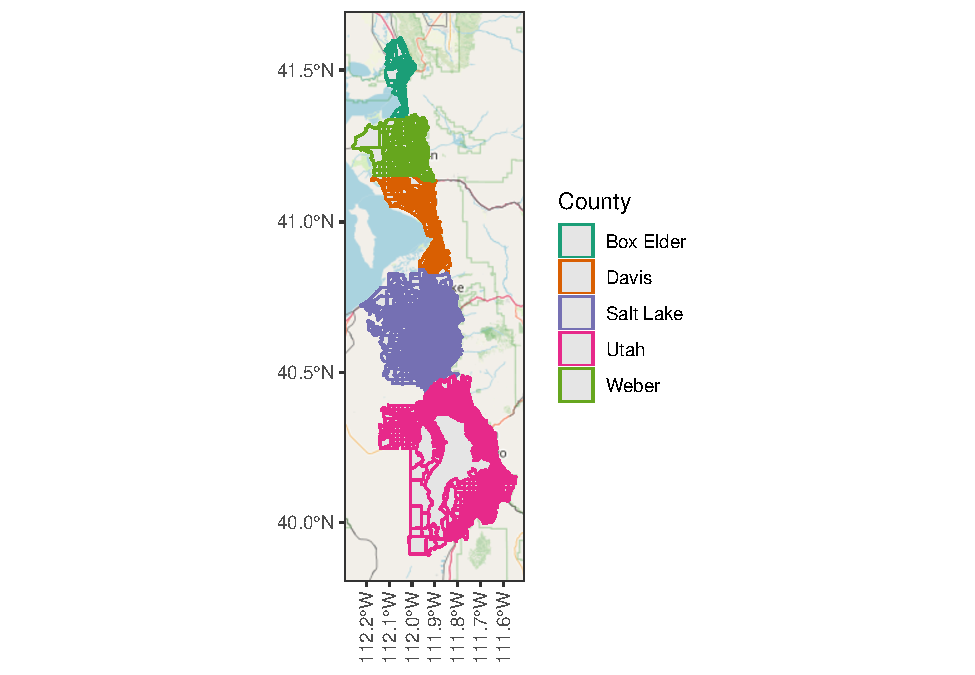
\includegraphics[width=480px]{thesis_files/figure-latex/figregion-1} 

}

\caption{The TAZs of each county in the region of study.}\label{fig:figregion}
\end{figure}

This extensive region was selected for the following reasons:

\begin{enumerate}
\def\labelenumi{\arabic{enumi}.}
\tightlist
\item
  There is substantial data that exists for this region. Having sufficient data points for each of the TAZs was essential to creating the inputs to ActivitySim and BEAM. The majority of the data used for this research was gathered and shared by Wasatch Front Regional Council (WFRC), the Metropolitan Planning Organization (MPO) of Salt Lake county.
\item
  There currently exists a need to analyze this region with a microsimulation tool, such as BEAM. Specifically, the Utah Transit Authority (UTA) wishes to understand which specific sub regions in the Salk Lake area will best serve new on-demand transit vehicles. In some future research, this specific question will be answered. Along this this question, having a microsimulation model of a region will prove to be an effective method to answering multiple transportation service questions in the future. To date, only one previous analysis of this region has been conducted with the BEAM software (Lant 2021).
\item
  The size and population within the study area are comparable to other regions around the United States. This means that the work completed in this research may be useful to other cities besides Salt Lake City.
\item
  The project researchers live in this region, and therefore have real life knowledge of how transportation works in the region. This allows the researchers to compare the results of the models with their own experiences, hopefully providing extra verification.
\end{enumerate}

Overall, the Salt Lake City, Utah region proved to be an effective location for this mode choice analysis research. After selecting the region of study, the next steps involved setting up and running ActivitySim.

\hypertarget{setting-up-and-running-activitysim}{%
\subsection{Setting up and Running ActivitySim}\label{setting-up-and-running-activitysim}}

Setting up and running ActivitySim for the Salt Lake region was based off example scenarios presented by ActivitySim (ActivitySim 2021). The entire process for setting up the activity-based model for this region is explained in the research done by Lant (2021). The research done by Lant (2021) was the basis to the work completed in this project.

However, a brief explanation of the setup of the activity-based model is explained in Section \ref{asiminput}. The two main steps behind creating an activity-based model for the Salt Lake region was creating corresponding input files and calibrating and validating the results.

\hypertarget{asiminput}{%
\subsubsection{Creating Input Files}\label{asiminput}}

ActivitySim requires the following three input files in order to run:

\begin{itemize}
\tightlist
\item
  A synthetic population of the agents within the study area.
\item
  A zonal socioeconomic data file describing the characteristics of each zone.
\item
  A set of skims that describe the cost and travel times of all modes between all zones.
\end{itemize}

The synthetic population is used to generate an entire population with specific individual details for each agent (like gender, age, income, vehicle ownership). Gathering individual information for all the agents in the region may be considered an invasion of privacy. So instead, a synthetic population is used. The synthetic population is a generated population with specific individual attributes that add up to the regional characteristics as a whole. The synthetic population was generated using a software called PopulationSim (PopulationSim 2021). To run PopulationSim a ``seed'' table and a set of ``targets'' were used. The ``seed'' table represented information about a subset of the population and the set of ``targets'' represented demographic data for smaller areas within the region (Lant 2021). Together, PopulationSim was able to simulate individual attributes for the approximate 2 million agents in the Salt Lake region.

The zonal socioeconomic data file stores zonal characteristics regarding household information, worker information, and other activity type information. This file specifically gives information on what types and how many types of activities may be found within a certain zonal region. This file was created using data from WFRC, Utah Automated Geographic Reference Center (AGRC 2021), and the synthetic population when necessary.

The third input to ActivitySim is detailed travel skims. Skims are large matrices showing travel times and costs between every set of zones within the area of study. Included in these skims were further details regarding differences in modes, distances, wait times, etc. (Lant 2021). The existing skims from WFRC were used along with some slight adjustments to fit the ActivitySim model.

\hypertarget{asimcal}{%
\subsubsection{Calibration and Validation}\label{asimcal}}

The calibration and validation of ActivitySim was conducted by Lant (2021). The purpose of the calibration and validation was to ensure the outputs generated by ActivitySim matched target regional values. Specifically trip productions, trip distributions, and mode choices were tested to match the given target values from WFRC's four-step model.

To validate the trip productions, total trips per county were compared between ActivitySim and WFRC target values. These trips were close to identical, with only a variation of 1.0 percent. The trip distributions were compared as well, with about a 4.0 percent margin of error. Overall, Lant (2021) shows that the trip productions and distributions of the ActivitySim model were a good representation of travel behavior, requiring no calibration.

The mode choice validation was difficult as the mode choice categories between WFRC and ActivitySim are vastly different. ActivitySim considers five trip mode choice alternatives whereas the WFRC model considers ten trip mode choice alternatives. However, ActivitySim does include ten tour mode choice alternatives. When comparing mode choice distributions, both the trip and tour distributions from ActivitySim were compared with the trip distributions of WFRC. Lant (2021) performs an in depth comparison between these values and found that ActivitySim under represents non-motorized university trips and over represents non-motorized work trips. In addition ActivitySim under represents shared ride trips for all tour purposes and does not accurately represent commuter rail and local bus trips for all tour purposes. overall, the mode choice model did not match closely with the WFRC targets, and required calibration.

Lant (2021) performed an in depth calibration across ActivitySim modes to minimize error with the WFRC target shares. The calibration process will not be explained in this research paper. Upon calibration, trip productions and distributions remained relatively unchanged, and therefore needed no calibration. Mode choice distributions were closer to target values as well. Overall, after some calibration the results of ActivitySim produced sufficiently accurate information to move forward with the research.

\hypertarget{setting-up-beam}{%
\subsection{Setting up BEAM}\label{setting-up-beam}}

After setting up, calibrating, and running the ActivitySim scenario for the Salt Lake region, the next step was setting up BEAM using the results of the ActivitySim model. BEAM requires a variety of input files, most of which are as follows:

\begin{itemize}
\tightlist
\item
  A person population and corresponding person attributes file.
\item
  A household population with household attributes file and a vehicle fleet file.
\item
  Vehicle types files explaining different person vehicle types, public transit vehicle types, and ride hailing vehicle information.
\item
  Transportation services including a mapable street network and a file including General Transit Feed Specification (GTFS) transit information.
\item
  Other minor input files.
\end{itemize}

The details behind these input files along with example tables of these files are discussed and shown in the following subsections.

\hypertarget{population-file}{%
\subsubsection{Population File}\label{population-file}}

The population file was created from the ActivitySim generated data. ActivitySim's main purpose is to generate daily activity patterns (DAPs) for each agent from the synthetic population. The DAPs generated by ActivitySim consists of all the activities that each agent within the population embark on during the day. Using the activity types, activity locations, activity durations, mode choices, departure and arrival times, and overall activity data, BEAM generated a population file along with a person attributes file.

The population file generated describes all the events and choices each agent embarks on within the plan. For example, the plans file defines each agents home location, their activity locations, their travel and activity times, their mode choices for each trip, etc. A subsection of this file is shown in Table \ref{tab:plans} to provide an example of some of its contents.

\begin{table}

\caption{\label{tab:plans}A Subset of the Population Plans}
\centering
\begin{tabular}[t]{rllrlrrr}
\toprule
ID & Mode & Type & End Time & Purpose & Household ID & LocaitonX & LocaitonY\\
\midrule
50 & NA & Home & 25668.0 & escort & 6 & 412577.3 & 4606340\\
50 & hov3 & NA & NA & escort & 6 & NA & NA\\
50 & NA & escort & 28170.0 & escort & 6 & 413589.0 & 4593487\\
50 & hov3 & NA & NA & escort & 6 & NA & NA\\
50 & NA & home & NA & escort & 6 & 412577.3 & 4606340\\
\addlinespace
51 & NA & Home & 36079.2 & work & 6 & 412092.6 & 4606274\\
51 & car & NA & NA & work & 6 & NA & NA\\
51 & NA & escort & 38109.6 & work & 6 & 418892.5 & 4567448\\
51 & car & NA & NA & work & 6 & NA & NA\\
51 & NA & work & 64998.0 & work & 6 & 424344.6 & 4537656\\
\addlinespace
51 & car & NA & NA & work & 6 & NA & NA\\
51 & NA & escort & 70578.0 & work & 6 & 409491.7 & 4552587\\
51 & car & NA & NA & work & 6 & NA & NA\\
51 & NA & home & NA & work & 6 & 412092.6 & 4606274\\
52 & NA & Home & 67010.4 & othdiscr & 6 & 412437.5 & 4606445\\
\bottomrule
\end{tabular}
\end{table}

The person attributes file describes individual characteristics such as income, gender, age, vehicle ownership, etc. A subsection of this file is shown in Table \ref{tab:peratt} to provide an example of some of its contents.

\begin{table}

\caption{\label{tab:peratt}A Subset of the Person Attributes File}
\centering
\begin{tabular}[t]{rrrrrrrrl}
\toprule
ID & Household ID & Age & Sex & VOT & TAZ & Income & Household Size & Auto Work Ratio\\
\midrule
50 & 6 & 50 & 2 & 9.518956 & 9 & 103337.40 & 10 & auto\_sufficient\\
51 & 6 & 56 & 1 & 9.518956 & 9 & 103337.40 & 10 & auto\_sufficient\\
52 & 6 & 35 & 2 & 9.518956 & 9 & 103337.40 & 10 & auto\_sufficient\\
53 & 6 & 23 & 2 & 9.518956 & 9 & 103337.40 & 10 & auto\_sufficient\\
54 & 6 & 15 & 2 & 6.349144 & 9 & 103337.40 & 10 & auto\_sufficient\\
\addlinespace
55 & 6 & 11 & 1 & 6.349144 & 9 & 103337.40 & 10 & auto\_sufficient\\
56 & 6 & 5 & 1 & 6.349144 & 9 & 103337.40 & 10 & auto\_sufficient\\
57 & 6 & 2 & 1 & 6.349144 & 9 & 103337.40 & 10 & auto\_sufficient\\
58 & 6 & 1 & 1 & 6.349144 & 9 & 103337.40 & 10 & auto\_sufficient\\
59 & 6 & 43 & 1 & 9.518956 & 9 & 103337.40 & 10 & auto\_sufficient\\
\addlinespace
599 & 58 & 71 & 1 & 8.431196 & 5 & 52461.37 & 9 & auto\_sufficient\\
600 & 58 & 63 & 2 & 8.431196 & 5 & 52461.37 & 9 & auto\_sufficient\\
601 & 58 & 35 & 2 & 8.431196 & 5 & 52461.37 & 9 & auto\_sufficient\\
602 & 58 & 23 & 2 & 8.431196 & 5 & 52461.37 & 9 & auto\_sufficient\\
603 & 58 & 16 & 1 & 5.623608 & 5 & 52461.37 & 9 & auto\_sufficient\\
\bottomrule
\end{tabular}
\end{table}

\hypertarget{household-and-vehicle-files}{%
\subsubsection{Household and Vehicle Files}\label{household-and-vehicle-files}}

ActivitySim generates three specific files: a households, a persons, and a trips file. The persons and trips files were used to construct the population plans file. The households file, however, was used to generate both the household and vehicle BEAM input files.

Within the BEAM households file, information such as household income, vehicle ownership, and the IDs of the agents and vehicles that correspond to each household ID is provided. Unfortunately, ActivitySim does not generate household coordinate locations, but does provide the TAZ in which the house presides. Therefore a random coordinate within the TAZ was assigned to each house. This household coordinate is then used to simulate starting and ending locations for each agent within their population plans file. An example of a subset of the households file that is used as an input to BEAM is shown in Table \ref{tab:house}.

\begin{table}

\caption{\label{tab:house}A Subset of the Households File}
\centering
\begin{tabular}[t]{rrrrrrl}
\toprule
Household ID & TAZ & Income & Household Size & LocationX & LocationY & Auto Work Ratio\\
\midrule
304379 & 1281 & 37362.029 & 8 & 419080.7 & 4498686 & auto\_sufficient\\
270209 & 1104 & 163050.420 & 4 & 426367.4 & 4506262 & auto\_sufficient\\
68811 & 555 & 17291.518 & 3 & 428645.4 & 4524432 & auto\_sufficient\\
83245 & 553 & 35756.388 & 2 & 426902.8 & 4523207 & no\_auto\\
373813 & 1516 & 54036.582 & 2 & 430560.8 & 4491969 & auto\_sufficient\\
\addlinespace
574302 & 341 & 68375.208 & 4 & 418986.0 & 4559249 & no\_auto\\
253735 & 1197 & 192125.910 & 2 & 431933.2 & 4504105 & auto\_sufficient\\
53111 & 473 & 21239.420 & 2 & 420837.4 & 4542079 & auto\_sufficient\\
366644 & 1481 & 13778.640 & 2 & 429353.8 & 4494406 & no\_auto\\
101334 & 666 & 9777.942 & 2 & 422532.8 & 4514347 & auto\_sufficient\\
\bottomrule
\end{tabular}
\end{table}

The vehicles file is quite simple in that it only includes information on the vehicle ID, vehicle type, and the household the vehicle belongs to. An example of a subset of the vehicles file that is used as an input to BEAM is shown in Table \ref{tab:veh}.

\begin{table}

\caption{\label{tab:veh}A Subset of the Vehicles File}
\centering
\begin{tabular}[t]{rlr}
\toprule
Vehicle ID & Vehicle Type & Household ID\\
\midrule
1 & CAR & 6\\
2 & CAR & 6\\
3 & CAR & 6\\
4 & CAR & 6\\
5 & CAR & 30\\
\addlinespace
6 & CAR & 30\\
7 & CAR & 30\\
8 & CAR & 30\\
\bottomrule
\end{tabular}
\end{table}

\hypertarget{vechile-types-files}{%
\subsubsection{Vechile Types Files}\label{vechile-types-files}}

In addition to the household and vehicle files, two vehicle type files are also needed to run BEAM. The first describes attributes that relate to each vehicle type. For example, some attributes that are included in the vehicle types file is the fuel efficiency, seating capacity, vehicle length, etc. An example of a subset of the vehicle types file that is used as an input to BEAM is shown in Table \ref{tab:vehtypes}.

\begin{table}

\caption{\label{tab:vehtypes}A Subset of the Vehicle Types Input File}
\centering
\begin{tabular}[t]{lrrrll}
\toprule
ID & Seats & Standing Room & Length (m) & Fuel & Vehicle Type\\
\midrule
BODY-TYPE-DEFAULT & 0 & 0 & 0.5 & Food & Body\\
BIKE-DEFAULT & 2 & 0 & 1.5 & gasoline & Bike\\
FAST-BIKE & 2 & 0 & 1.5 & gasoline & Bike\\
Car & 4 & 0 & 4.5 & gasoline & Car\\
CAR & 4 & 0 & 4.5 & gasoline & Car\\
\addlinespace
Car-rh-only & 4 & 0 & 4.5 & gasoline & Car\\
WAV & 6 & 0 & 4.5 & gasoline & Car\\
CAV & 4 & 0 & 4.5 & gasoline & Car\\
BEV & 4 & 0 & 4.5 & electricity & Car\\
PHEV & 4 & 0 & 4.5 & electricity & Car\\
\addlinespace
BUS-DEFAULT & 37 & 20 & 12.1 & diesel & MediumDutyPassenger\\
RAIL-DEFAULT & 801 & 2052 & 129.6 & diesel & MediumDutyPassenger\\
FERRY-DEFAULT & 149 & 0 & 26.0 & diesel & MediumDutyPassenger\\
SUBWAY-DEFAULT & 336 & 864 & 129.6 & electricity & MediumDutyPassenger\\
CABLE\_CAR-DEFAULT & 29 & 31 & 8.4 & electricity & MediumDutyPassenger\\
\addlinespace
TRAM-DEFAULT & 58 & 19 & 14.0 & electricity & MediumDutyPassenger\\
\bottomrule
\end{tabular}
\end{table}

A secondary vehicle types file exists that describes the nature of the ride hail fleet. One particular advantage to the microsimulation tool BEAM is its ability to model on-demand transit vehicles in a realistic manner. Part of creating realistic ride-hailing services is using an input file describing the nature of the fleet of ride-hail vehicles. An example of a subset of the ride-hail vehicle attributes file that is used as an input to BEAM is shown in Table \ref{tab:rhveh}. For this research project, the ride-hail file used was taken from an example BEAM scenario. In the future however, a ride hailing fleet file that accurately depicts the nature of ride hail vehicles in the Salt Lake region will be used. For this research it was not necessary to include, and so a default file was used instead.

\begin{table}

\caption{\label{tab:rhveh}A Subset of the Vehicle Types Input File}
\centering
\begin{tabular}[t]{llrrl}
\toprule
ID & Vehicle Type & Starting Point X & Starting Point Y & Shift Times\\
\midrule
rideHailVehicle-033000 & Car & 414692.0 & 4498566 & \{10:25200\}\\
rideHailVehicle-012301 & Car & 418969.2 & 4495377 & \{10:25200\}\\
rideHailVehicle-035201 & Car & 422864.0 & 4527397 & \{10:25200\}\\
rideHailVehicle-031400 & Car & 430458.0 & 4508789 & \{10:25200\}\\
rideHailVehicle-030800 & Car & 417063.9 & 4568028 & \{10:25200\}\\
\addlinespace
rideHailVehicle-016300 & Car & 415844.3 & 4544000 & \{10:25200\}\\
rideHailVehicle-033100 & Car & 408380.1 & 4550982 & \{10:25200\}\\
rideHailVehicle-061500 & Car & 436159.1 & 4474228 & \{10:25200\}\\
rideHailVehicle-032601 & Car & 420785.5 & 4484536 & \{10:25200\}\\
rideHailVehicle-015500 & Car & 444235.6 & 4452609 & \{10:25200\}\\
\addlinespace
rideHailVehicle-016400 & Car & 410876.3 & 4506167 & \{10:25200\}\\
rideHailVehicle-061400 & Car & 414579.1 & 4485811 & \{10:25200\}\\
rideHailVehicle-017601 & Car & 411338.4 & 4548806 & \{10:25200\}\\
rideHailVehicle-020700 & Car & 446697.0 & 4437390 & \{10:25200\}\\
rideHailVehicle-010500 & Car & 425560.0 & 4483818 & \{10:25200\}\\
\bottomrule
\end{tabular}
\end{table}

\hypertarget{transportation-services}{%
\subsubsection{Transportation Services}\label{transportation-services}}

BEAM requires two main files in order to provide transportation services to agents within the simulation. These two files are a GTFS file and a routable transportation network.

GTFS data is a common format that houses information relating to transportation schedules and transportation locations. Many public agencies publish transportation data in the GTFS format. The GTFS data used as the input to BEAM was obtained from UTA's mobility data feed from 2019 (UTA 2021). BEAM maps the GTFS data onto the highway network allowing agents to use both transportation and highway services interchangeably (Lant 2021).

A detailed routable road network for the study area was obtained from WFRC's travel demand model. After some manipulation, the network was cleaned of disconnections and filtered to include the correct attributes. Within the network, various attributes such as capacity, free flow speed, number of lanes, functional classification, direction, whether it is a one-way street, etc. were included. The network was constructed from a series of link and node combinations. The nodes represent intersections and activity locations whereas the links represent the roadways that connect each node. The links include the attributes of the network whereas the nodes include the coordinates. A detailed highway network of links and nodes allows BEAM to simulate traffic conditions in a more realistic manner.

Figure \ref{fig:network} displays the roadway network of the region of study. Figure \ref{fig:closent} displays a close up of roadway network system within Salt Lake City, Utah to show significant detail.

\begin{figure}

{\centering 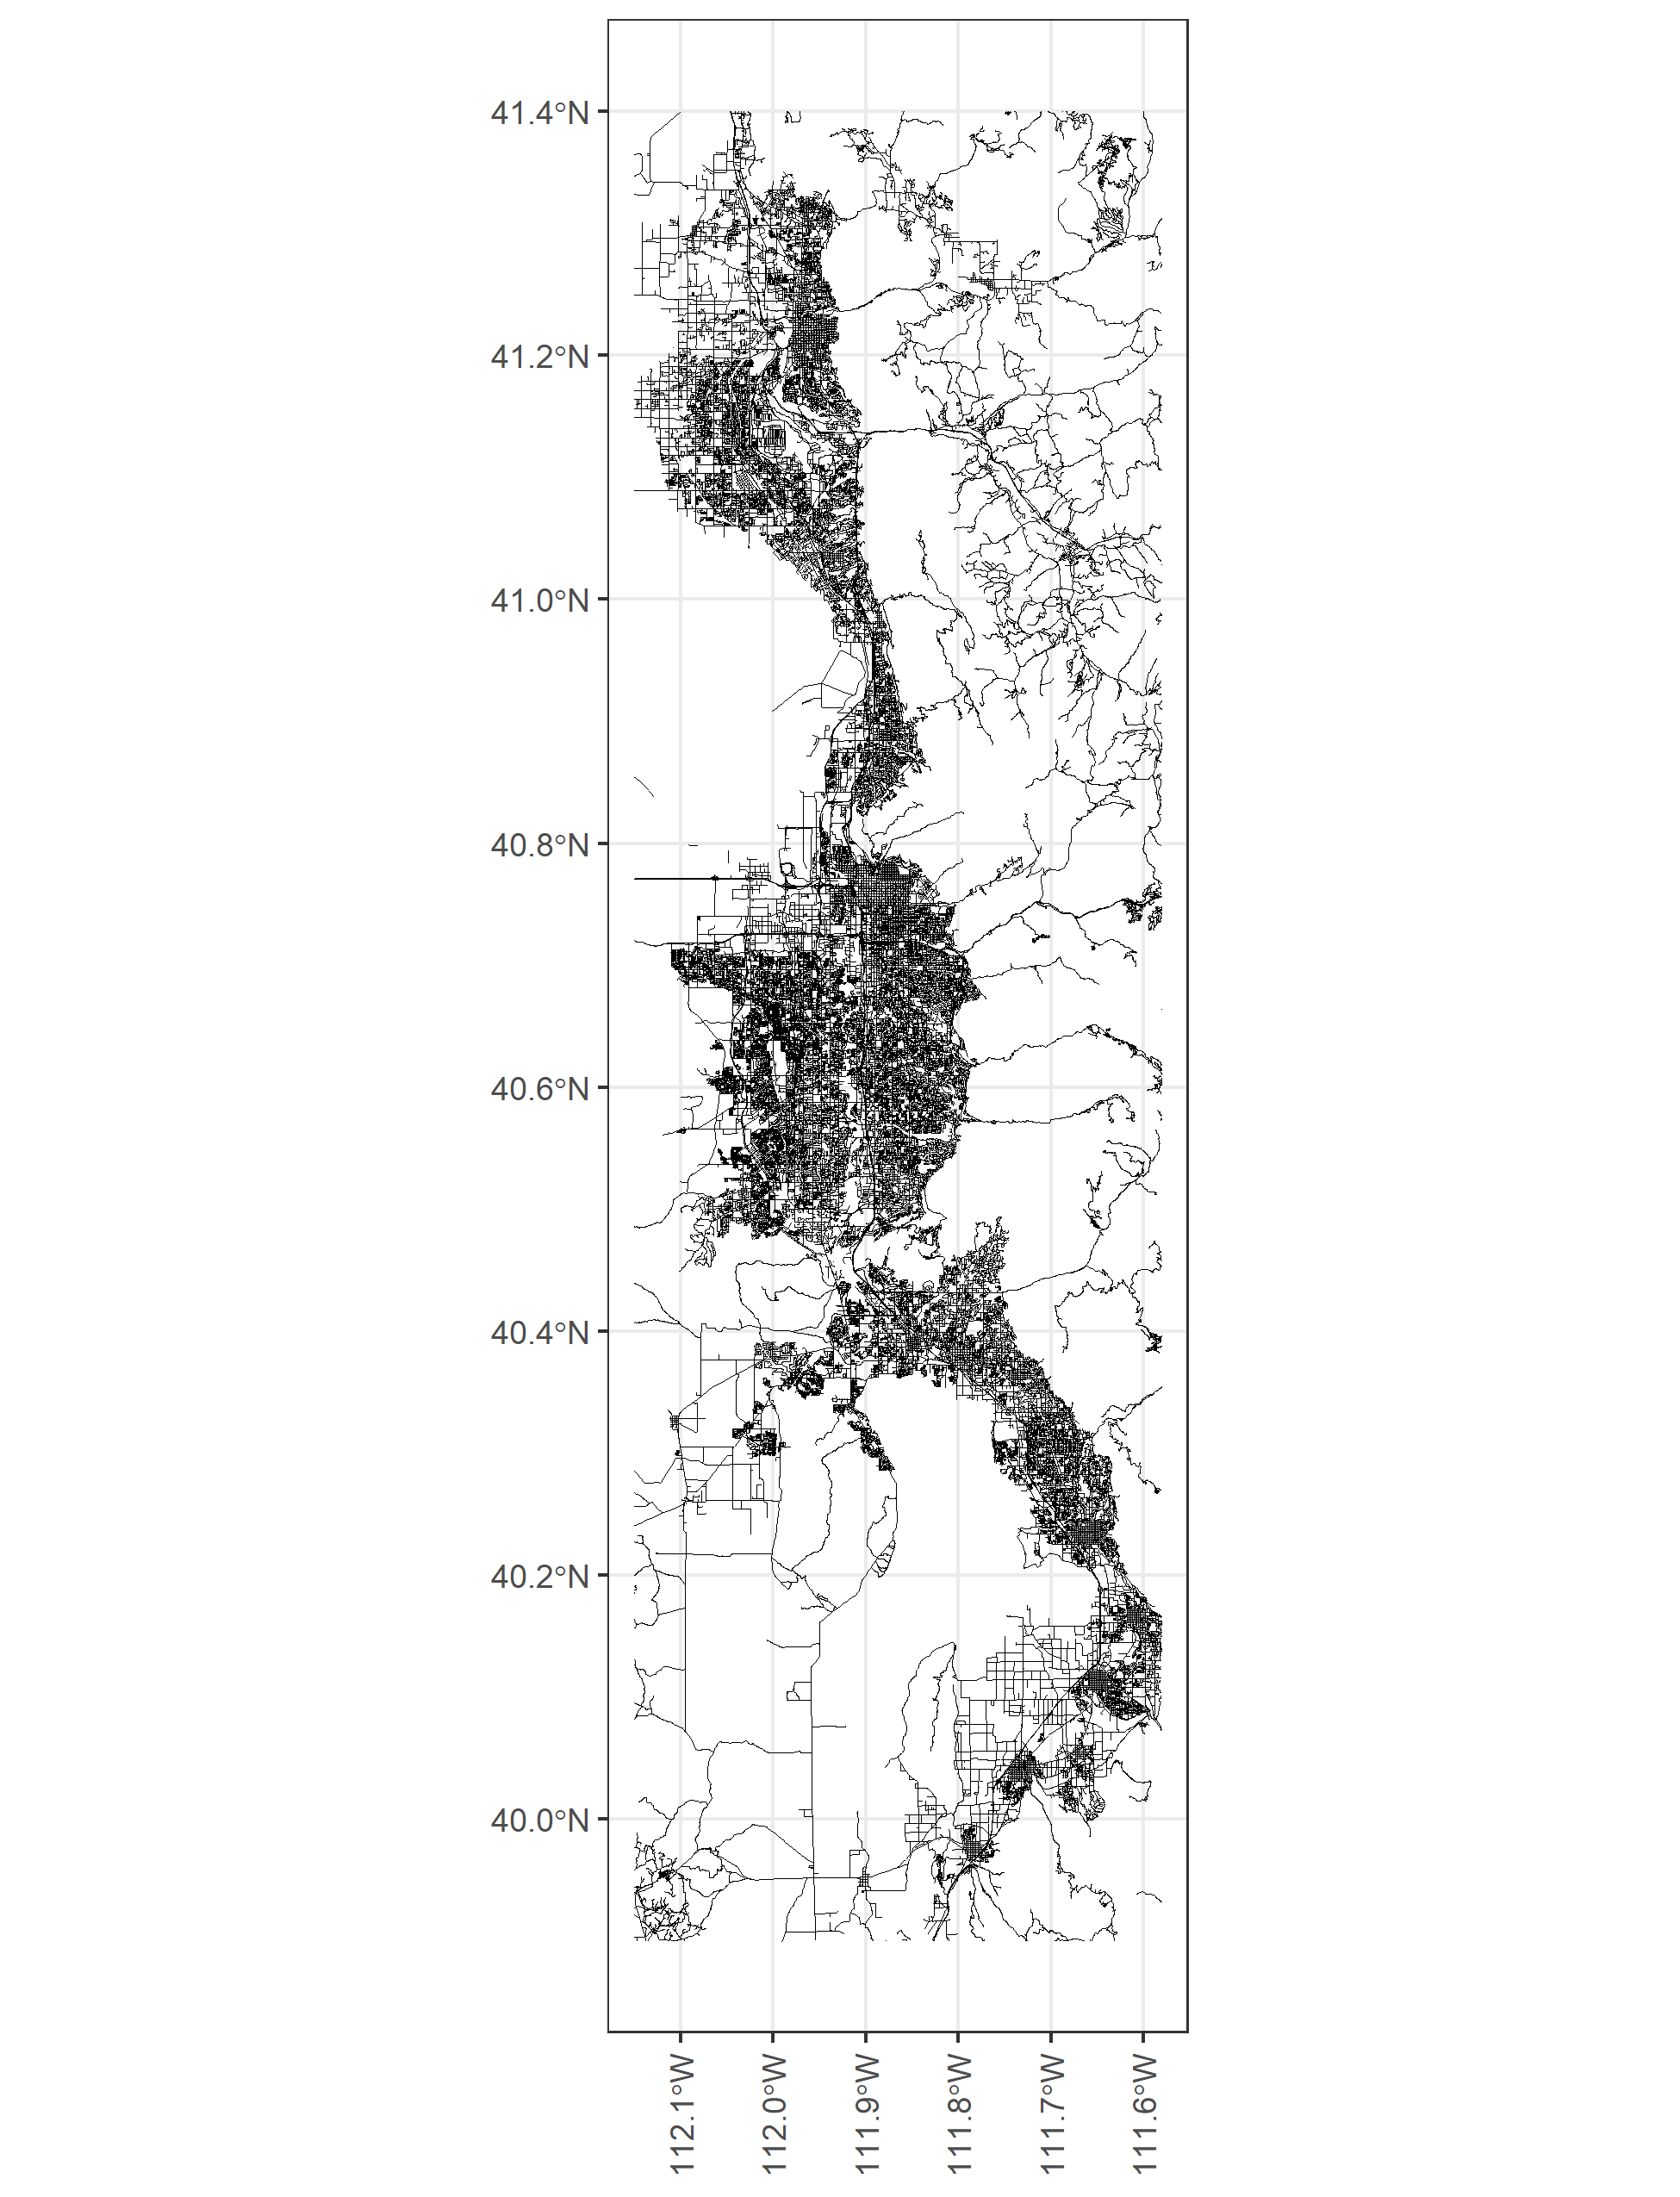
\includegraphics[width=480px]{pics/network} 

}

\caption{Transportation network for area of study.}\label{fig:network}
\end{figure}

\begin{figure}

{\centering 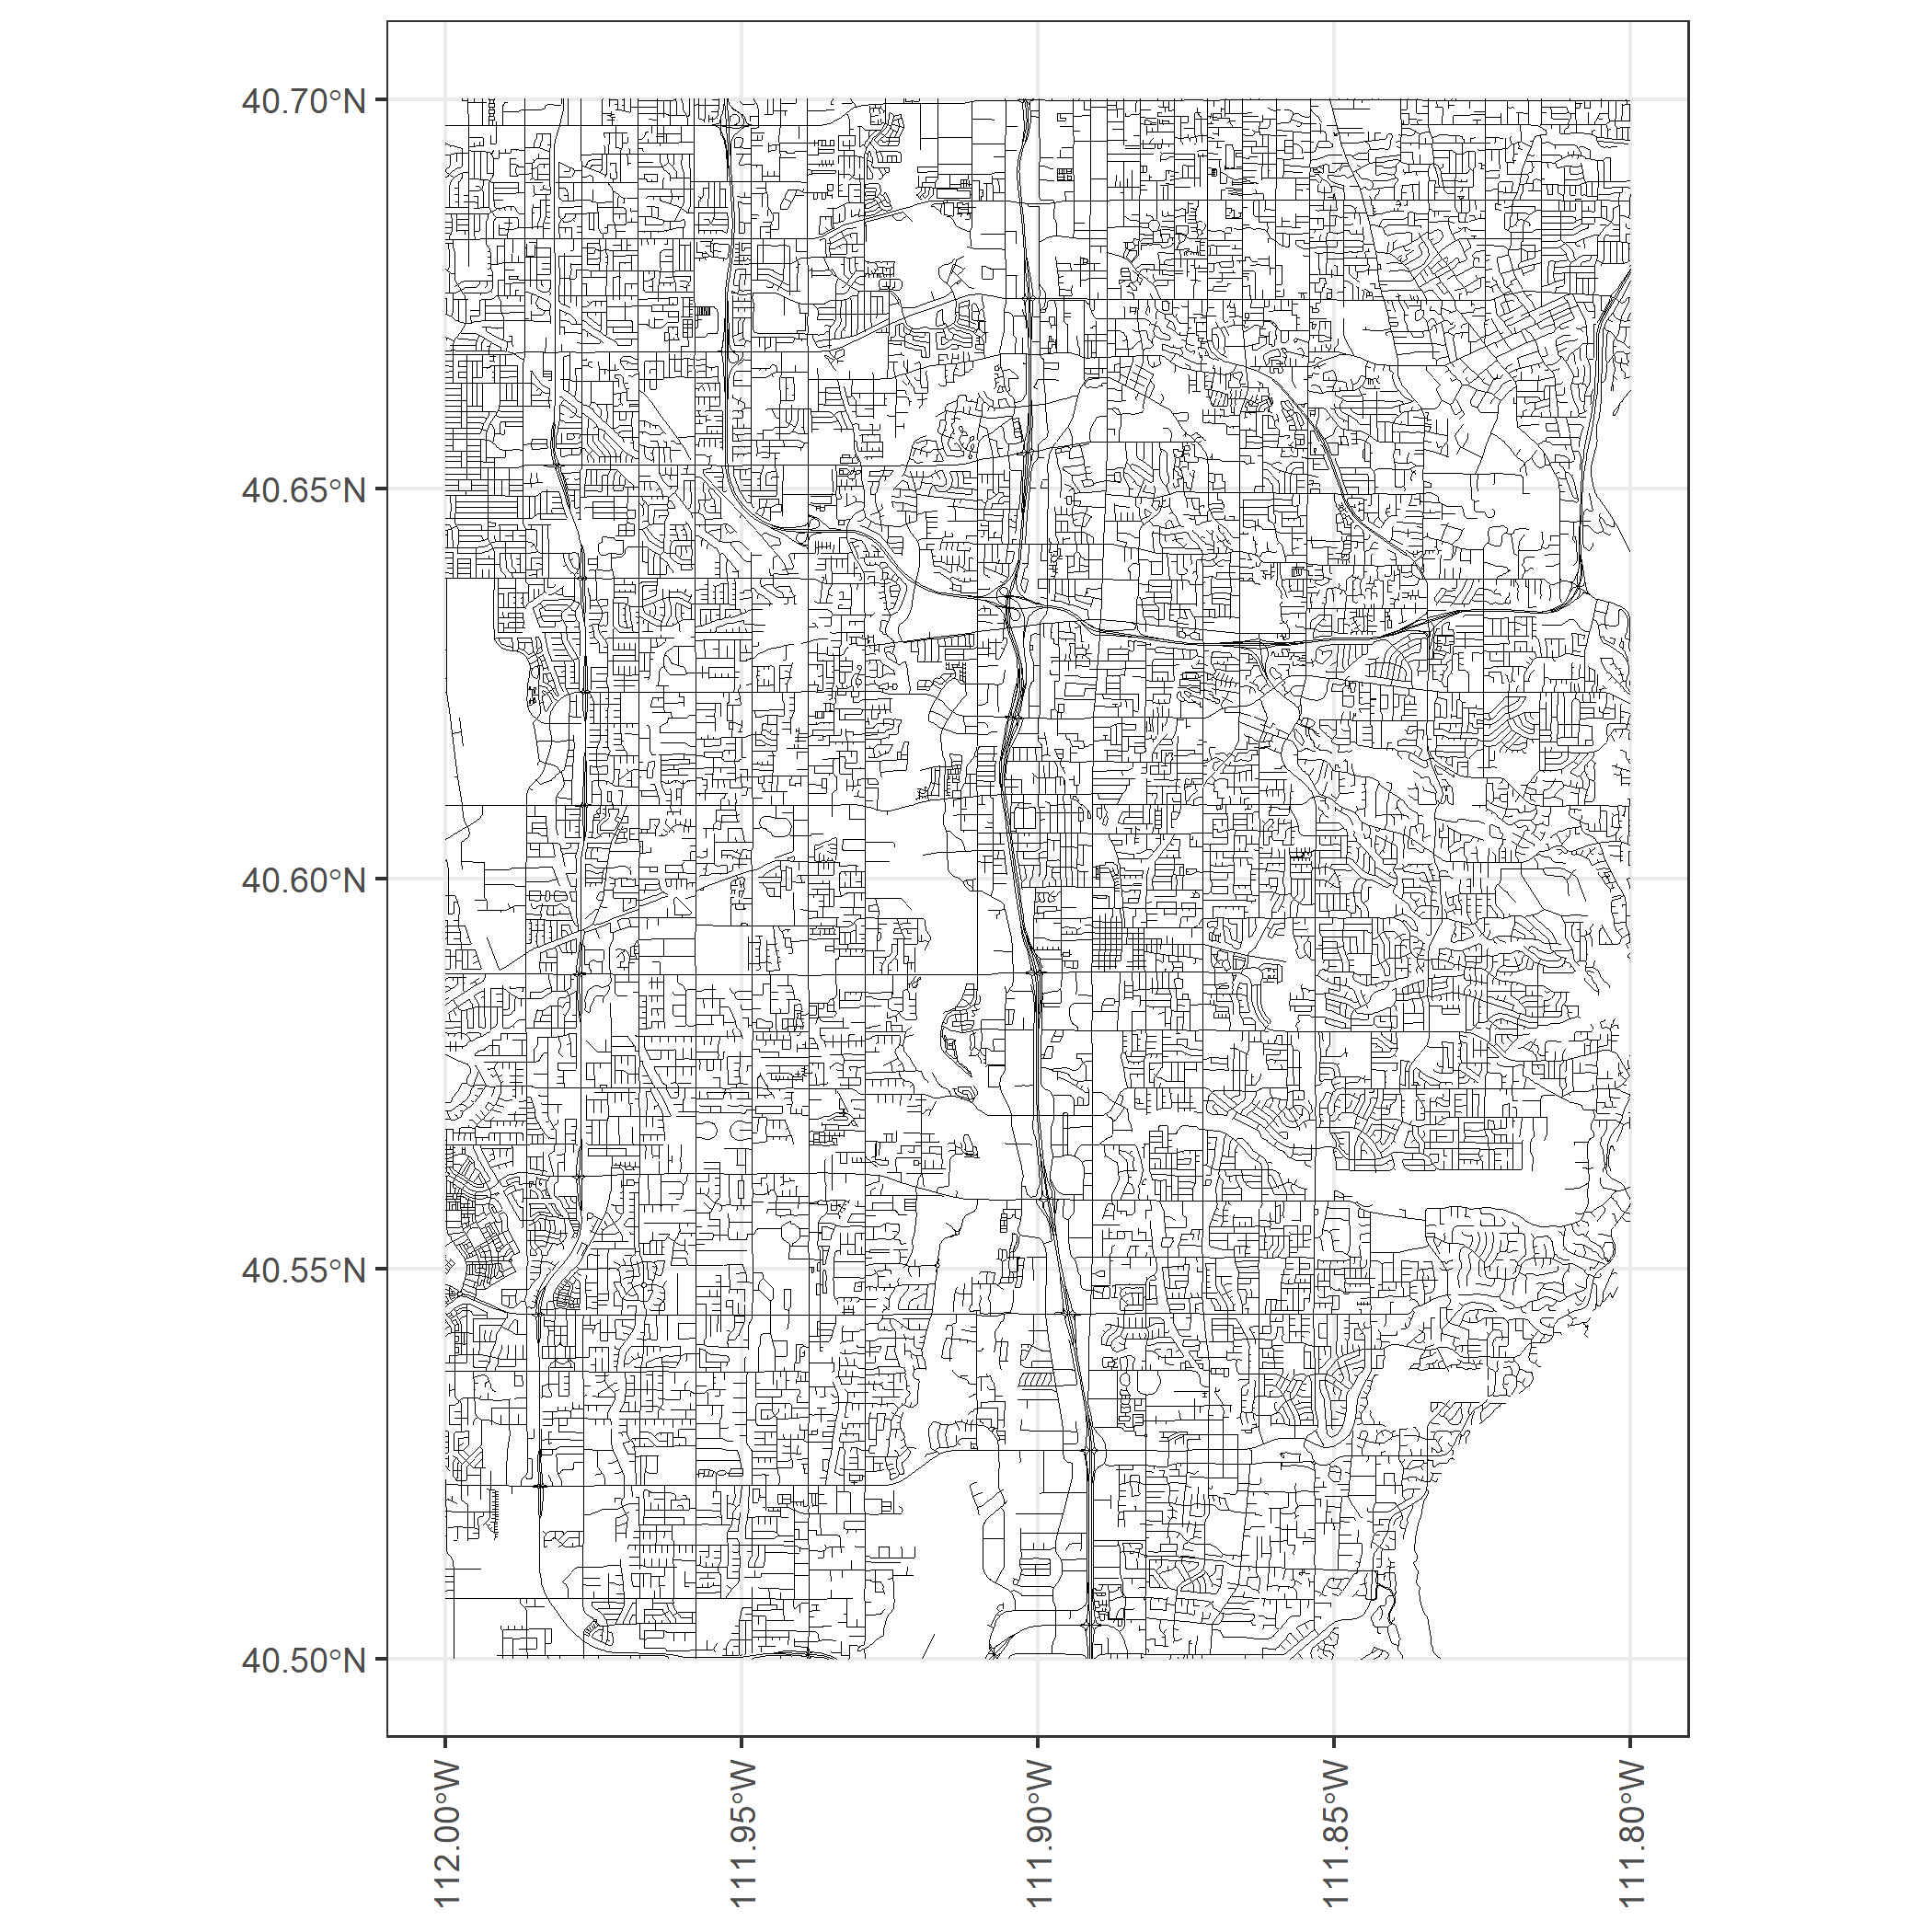
\includegraphics[width=480px]{pics/smallnetwork} 

}

\caption{Close up of the transportation network of Salt Lake City.}\label{fig:closent}
\end{figure}

\hypertarget{other-input-files}{%
\subsubsection{Other Input Files}\label{other-input-files}}

A variety of additional input files can be included to run the BEAM simulation. Not all the files will be mentioned, but a few of them include a configuration file, a parking file, a toll prices file, TAZ specific files, and mode choice utility parameter file. Except for the mode choice utility parameter file, details about these additional files will not be provided. The details behind the mode choice utility parameter file will be discussed in Section \ref{ute}.

\hypertarget{mbeam}{%
\section{Improved Mode Choice in BEAM}\label{mbeam}}

After creating the basic input files in order to run BEAM for the Salt Lake region, the next step was adjusting the mode choice model within BEAM itself. As discussed in Section \ref{lit7} BEAM's default mode choice model is a simple multinomial logit model calculated with minimal travel attributes. In Section \ref{lit4} it is discussed that ActivitySim's mode choice model is more comprehensive.

Changing the mode choice model within BEAM to become more consistent with that of ActivitySim's required some major adjustments to BEAM's internal code. Specifically, in this research BEAM's code was changed in three significant ways. Section \ref{purp} describes how choices were changed to be made using activity purpose values, Section \ref{ute} describes how additional attributes were inserted to the utility equation, and Section \ref{pool} describes how new modal alternatives were added to BEAM. Then, in Section\ref{algo} algorithms explaining BEAM's improved mode choice model is presented.

\hypertarget{purp}{%
\subsection{Purpose-based Decisions}\label{purp}}

The first major addition to BEAM's mode choice model to improve consistency with ActivitySim was to base mode choice decisions off of activity purposes. An activity purpose describes the primary activity of trips on a tour. Primary purposes are selected on a tour-based level. For this reason, the primary purpose is also referred to as the tour purpose. For example, if an agent were to go to the gym, then to work, and then return home, each trip on the work tour would have a primary purpose of ``work''. In this paper, tour purpose, primary purpose, activity purpose, and tour type are all used interchangeable to mean the same thing.

ActivitySim's mode choice coefficients vary between ten different tour purposes. These tour purposes are as follows:

\begin{itemize}
\tightlist
\item
  Work
\item
  University
\item
  School
\item
  Escort
\item
  Shopping
\item
  Eating Out
\item
  Social
\item
  Other Maintenance
\item
  Other Discretionary
\item
  At Work
\end{itemize}

To ensure the ability to distinguish between tour purpose values, it was necessary to adjust the population plans file to include a tour purpose trip-level attribute. Since ActivitySim bases decisions on activity purpose, it was simple to attach the attribute to the BEAM input plans file. As shown in Table \ref{tab:plans} a purpose attribute exists. After assigning this attribute to the plans, the next step was adjusting the BEAM code to read in a new attribute. By adjusting a few scripts relating to reading inputs, the primary purpose was able to be read into the BEAM software.

Once primary purpose values were present in the population plans, the next step was to design a new mode choice model within BEAM. In order to better understand the new code that was inserted into BEAM, three flow charts were constructed (See Figure \ref{fig:mnlflow}, Figure \ref{fig:lccmflow}, and Figure \ref{fig:tpcmflow}). In these flow charts inputs are displayed as folder icons, Java classes and methods are displayed as rectangles, and the result is displayed as an oval. These flow charts help display the code behind the BEAM's mode choice models. Understanding BEAM's default mode choice model and its obsolete Latent Class Choice Model (LCCM) are useful toward understanding how the new Tour Purpose Choice Model (TPCM) was constructed in the BEAM code.

\hypertarget{multinomial-logit-choice-model}{%
\subsubsection{Multinomial Logit Choice Model}\label{multinomial-logit-choice-model}}

Figure \ref{fig:mnlflow} shows the process behind BEAM's default mode choice model. As described in Section \ref{lit7}, by default BEAM calculates mode choices using a multinomial logit function with only a few attribute variables. In Figure \ref{fig:mnlflow} the flow of inputs and BEAM functions are shown. As shown, the inputs to the Mode Choice Calculator are the alternatives, person and household attributes, and the destination activity data.

\begin{figure}

{\centering 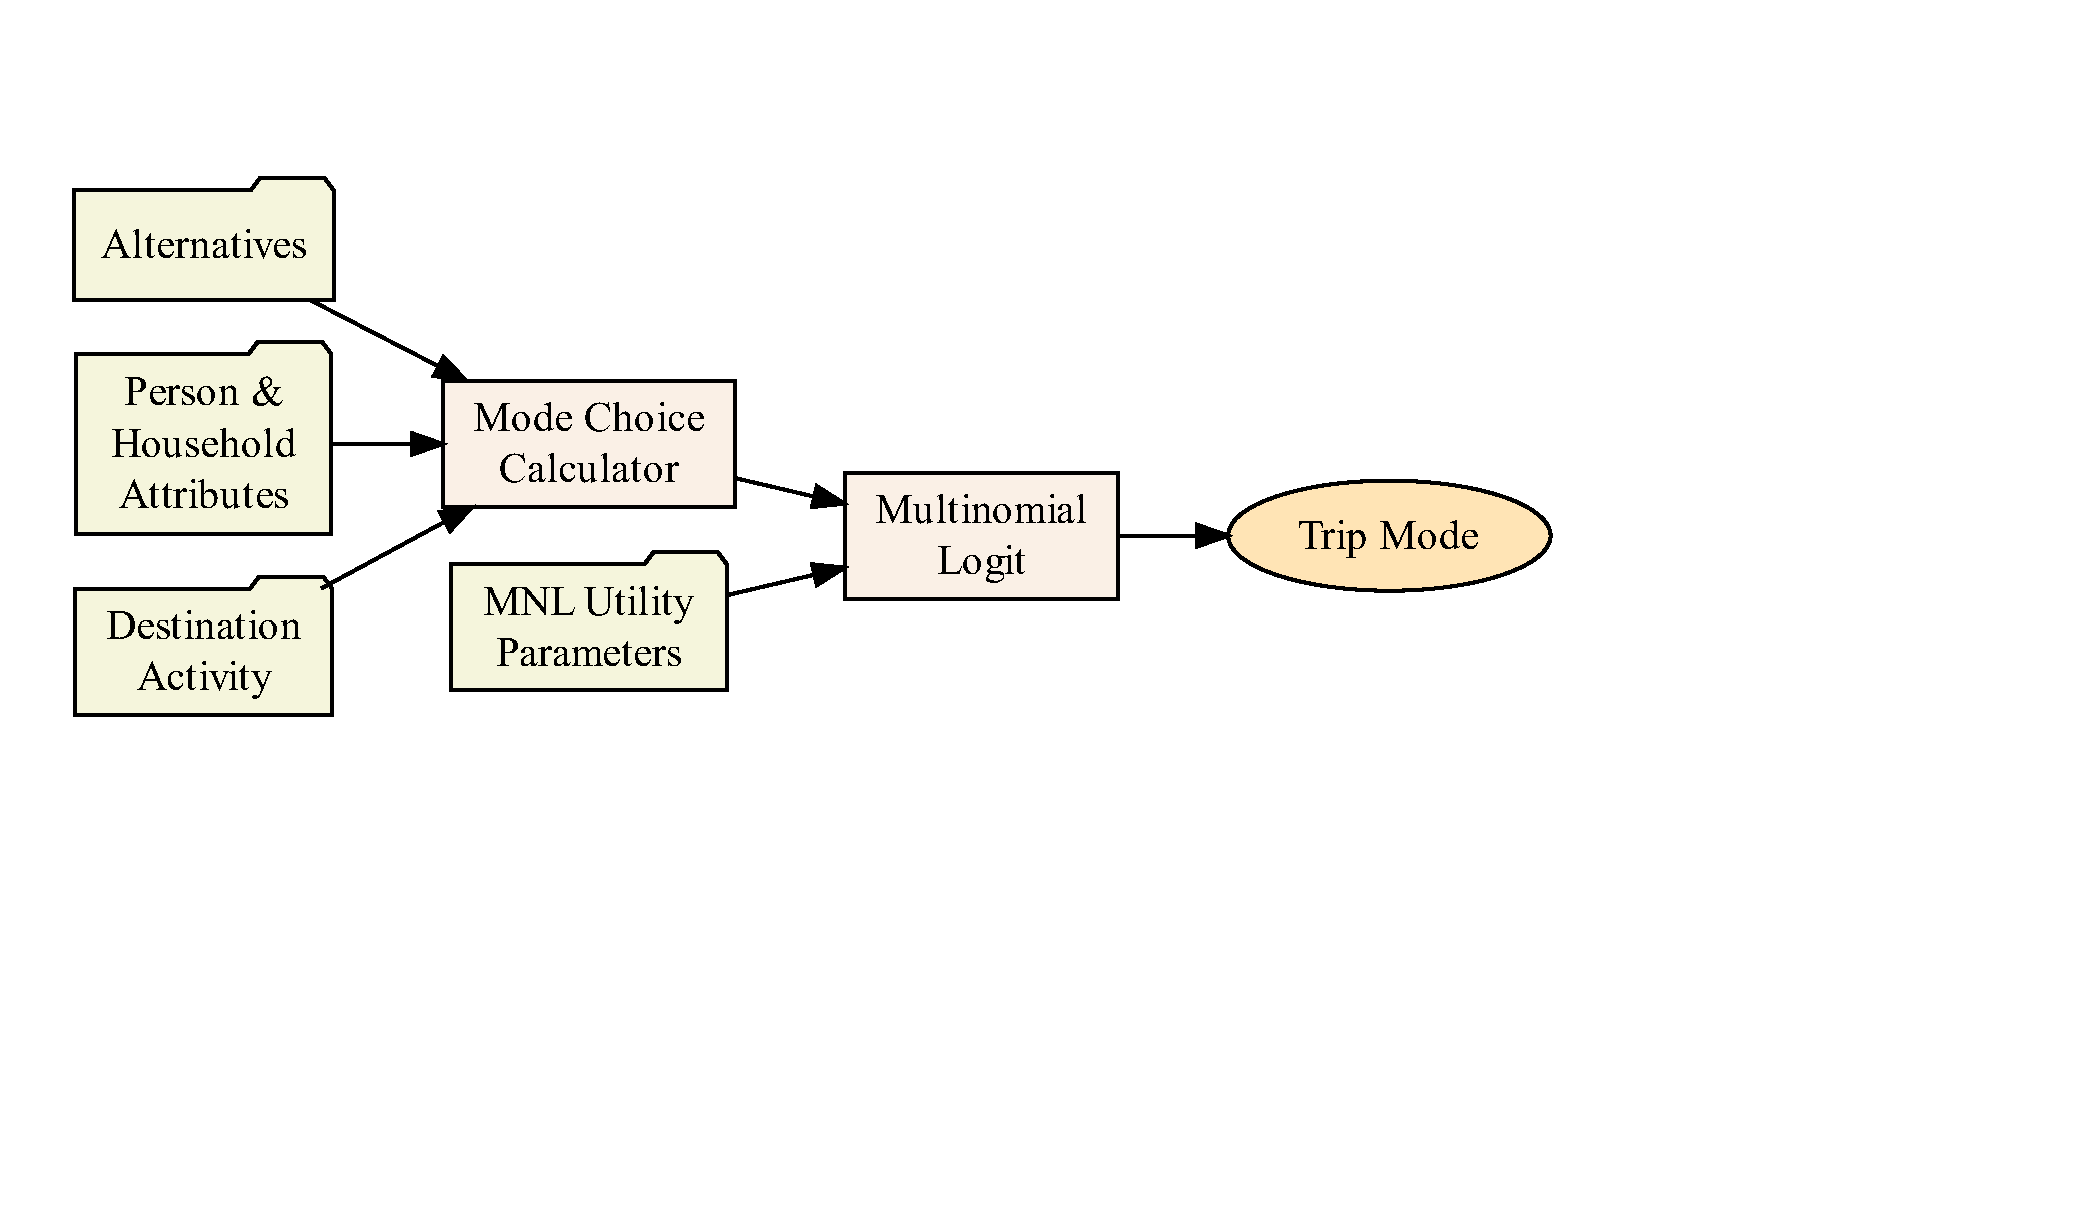
\includegraphics[width=600px]{thesis_files/figure-latex/mnlflow-1} 

}

\caption{BEAM code flow chart behind the default multinomial logit choice model.}\label{fig:mnlflow}
\end{figure}

The alternatives input represents a set of detailed travel itineraries that the agent can choose from. Within the alternatives variable, travel statistics, travel paths, travel modes, travel times, etc. are included. So as a result, the alternatives variable represents the modes in which the agent can choose from, while also including all the travel statistics needed to calculate the probability of selecting such mode. The next input is the person and household attributes variable. This variable includes all the information from the person attributes input file (See Table \ref{tab:peratt}) and the household attributes file (See Table \ref{tab:house}). Within the household attributes file some information from the vehicle inputs file is also included. The person and household attributes variable is also needed to calculate the probability of selecting such a mode. The last input is the destination activity data. This data simply includes additional information relating to the current trip and the destination activity. It is also useful to calculating the final mode choice.

The alternatives, person and household attributes, and destination activity are fed into the Mode Choice Calculator Java class. The purpose of this class is to organize the mode choice input data and organize it into a manner in which the choice model can process it efficiently. The Mode Choice Calculator class also houses some useful functions in the code used to calculate generalized travel time and the all day utility value.

The organized data from the Mode Choice Calculator along with the multinomial logit utility parameters are then sent to the multinomial logit choice model. The utility parameters in the default BEAM code are simply expressed in the configuration file. For each mode, an intercept, transit occupancy level, and transfer intercept/multiplier is specified. Then, within the multinomial logit choice model the utility value is calculated for each modal alternative. Those utility values are then sampled and one final mode is chosen!

\hypertarget{latent-class-choice-model}{%
\subsubsection{Latent Class Choice Model}\label{latent-class-choice-model}}

BEAM has an obsolete LCCM within its code structure. When BEAM was first being developed, the LCCM was how modal decisions were made. Part of creating the new Tour Purpose Choice Model was first to recreate and reboot the LCCM and second to change its structure slightly to base decisions off of tour purpose. For this reason, the structure behind the LCCM is presented. Figure \ref{fig:lccmflow} shows the flow of code for the LCCM.

\begin{figure}

{\centering 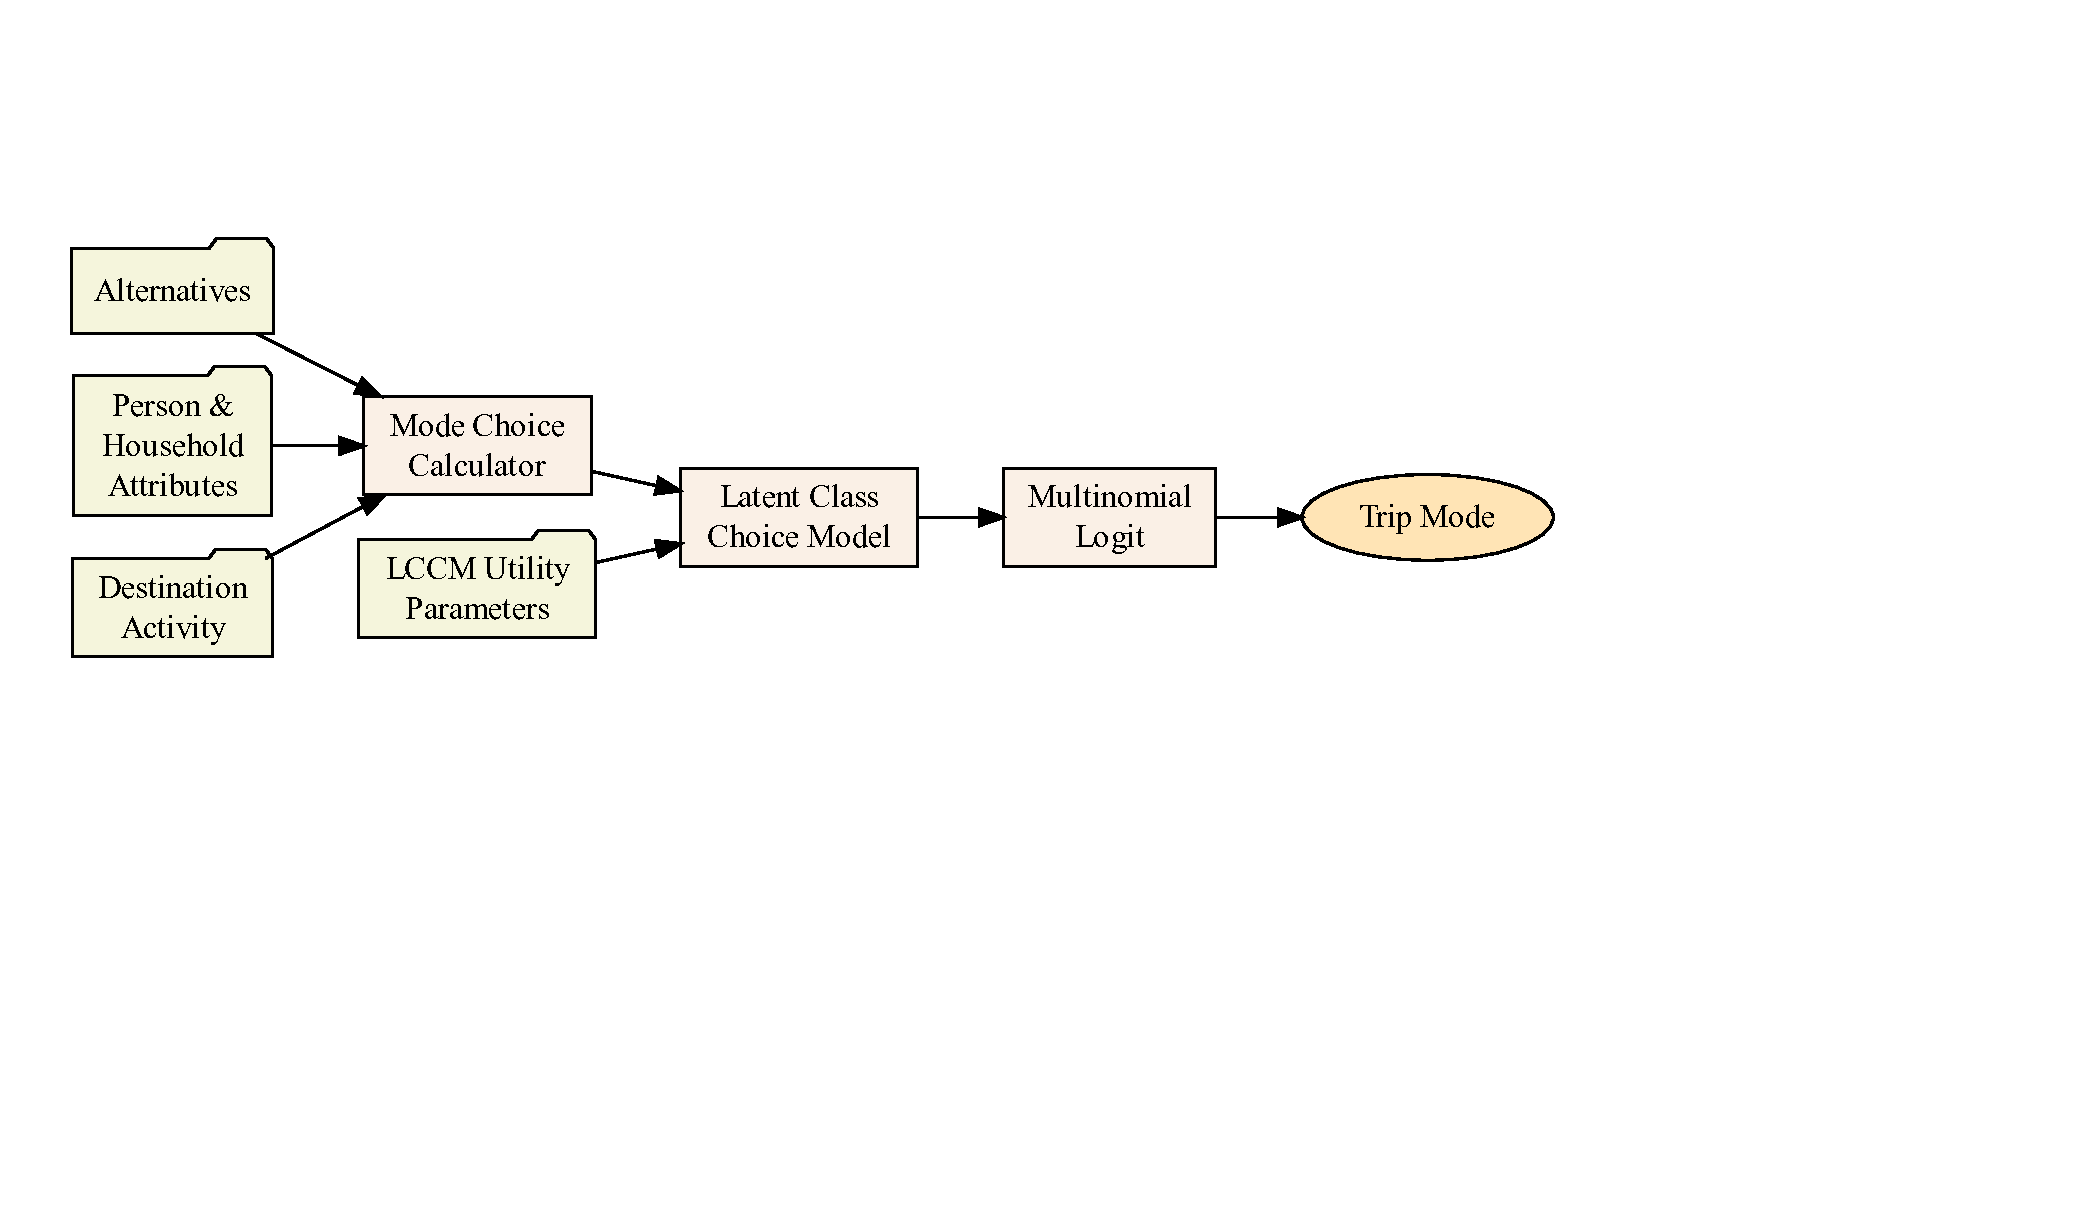
\includegraphics[width=650px]{thesis_files/figure-latex/lccmflow-1} 

}

\caption{BEAM code flow chart behind the latent class choice model.}\label{fig:lccmflow}
\end{figure}

Just like with the multinomial logit choice model, the same alternatives, person and household attributes, and destination activity inputs are fed into the Mode Choice Calculator. The Mode Choice Calculator then acts in a similar way to organize the data for further analysis. However, an additional step is taken where the information is sent to a Latent Class Choice Model Java class before it is sent to the Multinomial Logit Java class. Within the Latent Class Choice Model Java class, a few things happen. First, the LCCM Utility Parameters data file is read into the code and parsed. After parsing the data, the utility parameters are attached to each alternative and stored.

The LCCM Utility Parameters file includes mode choice coefficients relating to number of cars, household size, income, cost, time, and also alternative specific constants. The interesting part to the LCCM is that it calculates modes based off of which \emph{modality style} a particular agent is a part of. The \emph{modality style} represents the travel behavior of the individual. The LCCM code divides individuals up into one of the six groups or classes based on their \emph{modality style} travel behavior. The LCCM BEAM code provides two incredibly useful structures that are directly related to creating the TPCM. First, it provides a code structure that reads in a file storing specific and attribute related utility parameters. Second, it provides a code structure for storing these utility parameters into each alternative based on person/household attributes, travel statistics, and destination activity.

Interestingly enough, after the Latent Class Choice Model Java class reads in the utility information and stores it accordingly, it is sent to the same Multinomial Logit Java class. The overall utility value is calculated for each alternative and then are sampled down to a final mode choice!

\hypertarget{tour-purpose-choice-model}{%
\subsubsection{Tour Purpose Choice Model}\label{tour-purpose-choice-model}}

As mentioned previously, the TPCM was constructed off of the LCCM within BEAM. This means the first step to creating this model was fixing the LCCM and making the LCCM run correctly. With a few minimal code adjustments, and a lot of debugging, the LCCM was brought back to life. The final flow of code for the TPCM is presented in Figure \ref{fig:tpcmflow}.

\begin{figure}

{\centering 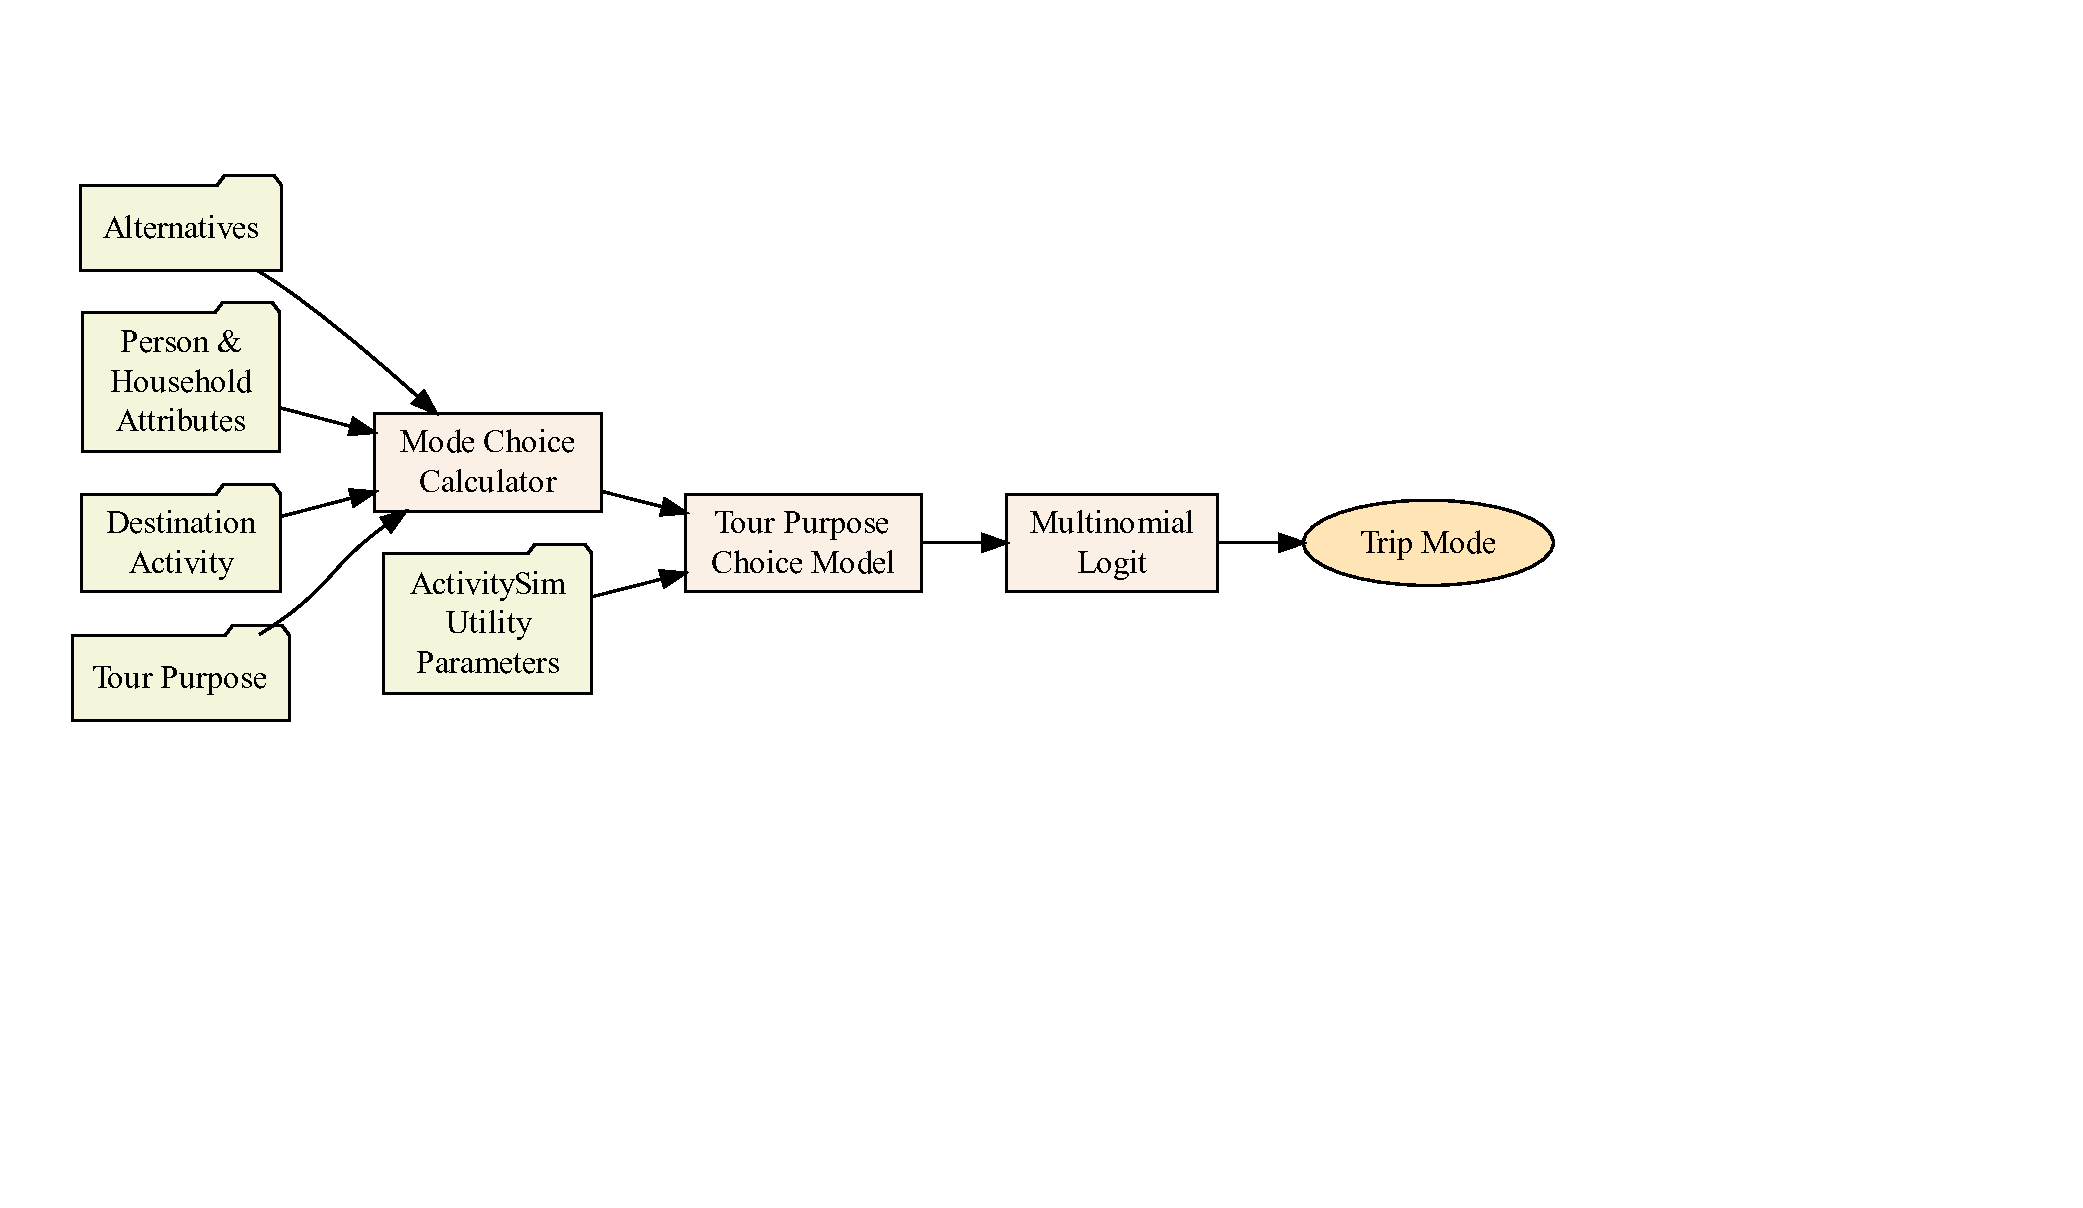
\includegraphics[width=650px]{thesis_files/figure-latex/tpcmflow-1} 

}

\caption{BEAM code flow chart behind the tour purpose choice model.}\label{fig:tpcmflow}
\end{figure}

The flow chart shows a very similar choice process as the LCCM, except that an additional input is sent to the Mode Choice Calculator. Obviously, the tour purpose value is necessary for the choice model and is therefore also sent to the Mode Choice Calculator. This input is only available, however, because it was attached to the population plans as explained previously.

In order to create the TPCM, two main steps were taken. First, a Tour Purpose Choice Model Java class was developed, mimicking how the code worked within the Latent Class Choice Model Java class. The TPCM was much more advanced than the LCCM, however, because instead of six classes to choose from there were ten activity purposes to choose from. In addition, instead of only needing a few travel statistics to do the mode choice, the TPCM included 25 different path, person, and location type variables. The second step toward creating the TPCM was to develop an input csv file that included all the utility parameter values from ActivitySim. These additional attributes used in the utility equation are discussed in Section \ref{ute}.

Overall, the Tour Purpose Choice Model Java class performed similarly to the Latent Class Choice Model Java class. It was able to parse the input utility parameters, attach those values to the alternatives, as well as calculate the travel statistics for all 25 travel variables. To do this, an additional class was built to calculate each of the travel variables. The final mode choice was determined in the same manner as well. These alternatives were sent to the Multinomial Logit Java class where their modal utilities were calculated and sampled. The sampling then determined a final mode choice for each individual.

\hypertarget{ute}{%
\subsection{Additional Attributes in Utility Equation}\label{ute}}

Equally important to developing the tour purpose choice model code structure within BEAM was to develop a consistent mode choice utility function. As explained in Section \ref{lit4} ActivitySim bases its mode choice off of an abundance of path, person, and location type variables. Therefore, most of these path, person, and location type variables were inserted into the BEAM structure and used to calculate mode choice. The travel statistics for each variable were calculated within the TPCM code and the coefficient and intercept parameter values were included using an input file.

The input file for the utility calculation included every combination of variable, mode, and purpose. For example, what is the cost coefficient for a drive transit trip on a school tour? With 25 different variables, 11 different modes, and 10 different tour purposes, a total of 3251 parameter values existed! Of course, a large portion of these combinations were left blank. (For example, the walk distance variable was only applied to walk type modes.) These parameter values were obtained from a variety of sources.

The alternate specific constants were obtained from the utility values used in the example\_mtc scenario from the ActivitySim software (ActivitySim 2021). These constants were used in the initial stages of modeling, but were then updated and calibrated to the Salt Lake Region in Section \ref{clib}. The majority of the coefficient values were obtained from the tour mode choice coefficients from MTC (2012). Since BEAM's mode choice is trip-based however, all these tour-based coefficients were multiplied by two and then used as trip-based coefficients. The trip-based coefficients from MTC (2012) were not used because they did not provide the same level of precision and thoroughness as the tour-based coefficients. Tour values were hence doubled as to better represent trip characteristics. In places where coefficients and constants did not exist for certain modes, the values of its most similar mode were used instead, sometimes with slight adjustments. For example, the bike transit constants did not exist so the walk transit values were used instead of leaving its values empty. Below, a list of the path, person, and location variables used to calculate the modal utility is shown. Not all 25 variables are listed since some of the variables describe a group of variables.

\begin{itemize}
\tightlist
\item
  \emph{Path Variables}: Number of Transfers, Vehicle Time, Egress Time, Wait Time, Origin to Transit Proximity, Destination to Transit Proximity, Walking Distance, Biking Distance, and Driving Distance
\item
  \emph{Person Variables}: Cost, Age, Household Size, and Vehicle to Worker Ratio
\item
  \emph{Location Variables}: Zonal Destination Index and Central Business District
\end{itemize}

In addition, Table \ref{tab:asimvals} shows a subsection of the input file with only the cost variable coefficients provided. The purpose of showing this table is to help understand how extensive the choice model was. Within the table it is clear to see that variation exists between tour purpose, modal alternative, and variable type. Only three modal alternatives are provided in the table.

\begin{table}

\caption{\label{tab:asimvals}Cost coefficient values for some modes from the utility parameters csv file}
\centering
\begin{tabular}[t]{lllllr}
\toprule
Variable Type & Variable & Alternative & Units & Tour Purpose & Value\\
\midrule
Person & cost & car & util/min & work & -0.026\\
Person & cost & car & util/min & univ & -0.044\\
Person & cost & car & util/min & school & -0.044\\
Person & cost & car & util/min & escort & -0.036\\
Person & cost & car & util/min & shopping & -0.036\\
\addlinespace
Person & cost & car & util/min & eatout & -0.036\\
Person & cost & car & util/min & othmaint & -0.036\\
Person & cost & car & util/min & social & -0.036\\
Person & cost & car & util/min & othdiscr & -0.036\\
Person & cost & car & util/min & atwork & -0.038\\
\addlinespace
Person & cost & ride\_hail & util/min & work & -0.026\\
Person & cost & ride\_hail & util/min & univ & -0.044\\
Person & cost & ride\_hail & util/min & school & -0.044\\
Person & cost & ride\_hail & util/min & escort & -0.036\\
Person & cost & ride\_hail & util/min & shopping & -0.036\\
\addlinespace
Person & cost & ride\_hail & util/min & eatout & -0.036\\
Person & cost & ride\_hail & util/min & othmaint & -0.036\\
Person & cost & ride\_hail & util/min & social & -0.036\\
Person & cost & ride\_hail & util/min & othdiscr & -0.036\\
Person & cost & ride\_hail & util/min & atwork & -0.038\\
\addlinespace
Person & cost & walk\_transit & util/min & work & -0.026\\
Person & cost & walk\_transit & util/min & univ & -0.044\\
Person & cost & walk\_transit & util/min & school & -0.044\\
Person & cost & walk\_transit & util/min & escort & -0.036\\
Person & cost & walk\_transit & util/min & shopping & -0.036\\
\addlinespace
Person & cost & walk\_transit & util/min & eatout & -0.036\\
Person & cost & walk\_transit & util/min & othmaint & -0.036\\
Person & cost & walk\_transit & util/min & social & -0.036\\
Person & cost & walk\_transit & util/min & othdiscr & -0.036\\
Person & cost & walk\_transit & util/min & atwork & -0.038\\
\bottomrule
\end{tabular}
\end{table}

The observable utility equation for the new tour purpose choice model can be divided up into three sub-equations. Equation \eqref{eq:tpcmpath} shows the Path type variable part of the TPCM utility equation. Equation \eqref{eq:tpcmperson} shows the Person type variable part of the TPCM utility equation. Equation \eqref{eq:tpcmloc} shows the Location type variable part of the the TPCM utility equation. The full TPCM utility equation, however, is the combination of path, person, and location type variables, as displayed in Equation \eqref{eq:tpcmall}.

\hypertarget{path-type-utility-equation}{%
\subsubsection{Path Type Utility Equation}\label{path-type-utility-equation}}

\begin{equation}
  V_j = \beta_{t_v}(t_v) + \beta_{t_w}(t_w) + \beta_{t_e}(t_e) + \beta_{tr_p}(tr_p) + \beta_{xfer}(xfer) + \beta_{w_{dis}}(w_{dis}) + \\ \beta_{b_{dis}}(b_{dis}) + \beta_{d_{dis}}(d_{dis}) \label{eq:tpcmpath}
\end{equation}

where

\begin{itemize}
\tightlist
\item
  \(j\) is the modal alternative,
\item
  \(t_v\) is the in vehicle travel time (mins),
\item
  \(t_w\) is the wait time (mins),
\item
  \(t_e\) is the egress time (mins),
\item
  \(tr_p\) is the proximity to transit (miles),
\item
  \(xfer\) is the number of transfers,
\item
  \(w_{dis}\) is the walk distance (miles),
\item
  \(b_{dis}\) is the bike distance (miles),
\item
  \(d_{dis}\) is the drive distance (miles),
\item
  \(\beta_{tr_p}\) differs between origin/destination and length, and
\item
  \(\beta_{w_{dis}}\), \(\beta_{b_{dis}}\), and \(\beta_{d_{dis}}\) differ between lengths.
\item
  \emph{Note:} All \(\beta\) values differ between mode and tour purpose.
\end{itemize}

\hypertarget{person-type-utility-equation}{%
\subsubsection{Person Type Utility Equation}\label{person-type-utility-equation}}

\begin{equation}
  V_j = ASC_{auto} +  \beta_{c}(c) + \beta_{ag}(ag) \label{eq:tpcmperson}
\end{equation}

where

\begin{itemize}
\tightlist
\item
  \(j\) is the modal alternative,
\item
  \(ASC_{auto}\) is the alternative specific constant that differs between modal alternative and auto ownership dependency,
\item
  \(c\) is the cost, and
\item
  \(ag\) is the age grouping (if the person is between 0-10 or 16-19 years old).
\item
  \emph{Note:} All \(\beta\) values differ between mode and tour purpose.
\end{itemize}

\hypertarget{location-type-utility-equation}{%
\subsubsection{Location Type Utility Equation}\label{location-type-utility-equation}}

\begin{equation}
  V_j = \beta_{zdi}(zdi) + \beta_{cbd}(cbd) \label{eq:tpcmloc}
\end{equation}

where

\begin{itemize}
\tightlist
\item
  \(j\) is the modal alternative
\item
  \(zdi\) is the zonal density index,
\item
  \(cbd\) is a classifier for zones labeled as central business district, and
\item
  \(\beta_{zdi}\) differs between origin/destination.
\item
  \emph{Note:} All \(\beta\) values differ between mode and tour purpose.
\end{itemize}

\hypertarget{beams-new-consistent-utility-equation}{%
\subsubsection{BEAM's New Consistent Utility Equation}\label{beams-new-consistent-utility-equation}}

\begin{equation}  
  V_j = Eq:4.1 + Eq:4.2 + Eq:4.3 \label{eq:tpcmall}
\end{equation}

where

\begin{itemize}
\tightlist
\item
  \(j\) is the modal alternative.
\end{itemize}

When comparing Equation \eqref{eq:tpcmall} with BEAM's default equation in Equation \eqref{eq:beammnl}, it is clear that multiple more travel variables are used to calculate the utility value. When comparing this Equation \eqref{eq:tpcmall} with the ActivitySim equations in Section \ref{lit4}, most of the same variable are used. By using most of the path, person, and location type variables to calculate the mode choice, the TPCM calculates utility in a consistent manner with ActivitySim. In addition, all utility values differ by tour purpose, making it almost identical to ActivitySim's trip-based mode choice.

It is important to note that BEAM's internal code is built on a trip-based level, and so no overarching tour mode choice was determined before trip mode choice. It was outside the scope of this project to adjust BEAM's structure to include a tour mode choice model. As a result, the mode choice consistency only exists on the trip-based mode choice level. Hopefully, in the future a consistent tour-based mode choice can be inserted into BEAM as well.

\hypertarget{pool}{%
\subsection{Carpool Alternatives}\label{pool}}

After designing a tour purpose choice model within BEAM and extending the mode choice utility equation, more consistency with ActivitySim was achieved by adding additional modal alternatives. BEAM by default includes nine modal alternatives. ActivitySim, however has eight upper level mode choices and 18 total mode choices. The lower level mode choices include distinctions between car and carpool modes being paid or not, and five different types of transit modes. For simplicity, BEAM's modes will be compared to ActivitySims upper level mode choice categories. Figure \ref{fig:venn} shows a venn diagram of how the modes compare between BEAM and ActivitySim.

\begin{figure}

{\centering 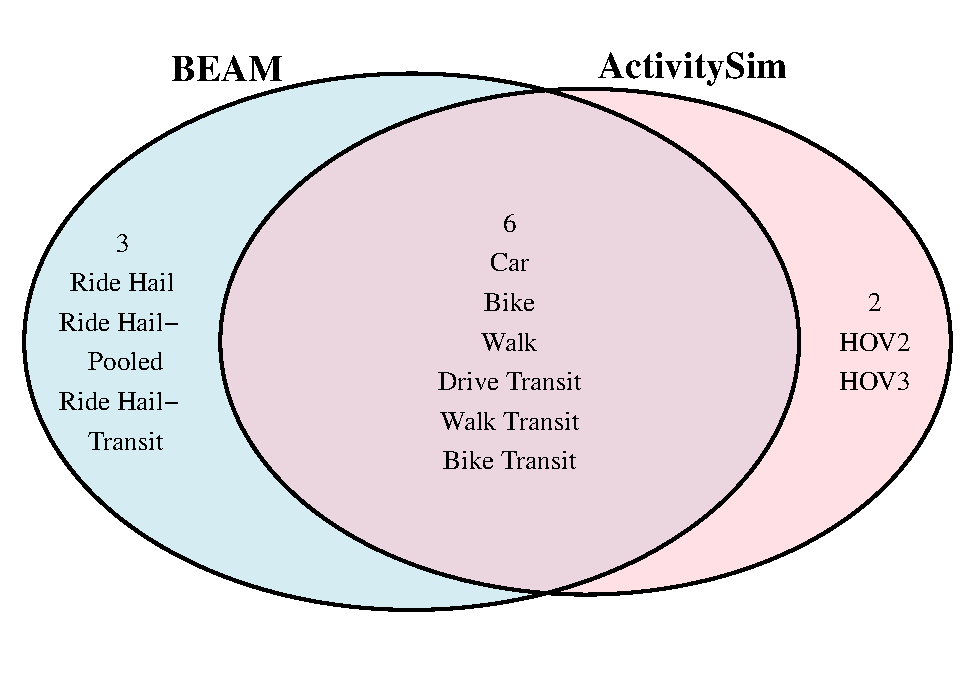
\includegraphics{thesis_files/figure-latex/venn-1} 

}

\caption{A comparison between BEAM and ActivitySim's modal alternatives.}\label{fig:venn}
\end{figure}

As seen in Figure \ref{fig:venn}, both BEAM and ActivitySim include car, bike, walk, and various types of transit modes. BEAM includes ride hailing modal alternatives whereas ActivitySim includes carpooling alternatives (HOV2 and HOV3). HOV2 means High Occupancy Vehicle with 1 passenger (2 people in the vehicle) and HOV3 means High Occupancy Vehicle with 2 or more passengers (at least 3 people in the vehicle). Both HOV2 and HOV3 simply represent the option to carpool. Therefore, to create more consistency with ActivitySim, carpooling/HOV alternatives were added into the BEAM mode choice model.

Four new carpooling alternatives were added to BEAM: HOV2, HOV2\_TELEPORTATION, HOV3, and HOV3\_TELEPORTATION. HOV2 and HOV3 were coded to act identical to car modes. They were mapped to the network and thus could add to congestion. Their travel statistics were also calculated in the same way as for car modes. Agents who selected HOV2 or HOV3 were represented as the drivers of the carpooling cars. HOV2\_TELEPORTATION and HOV3\_TELEPORTATION modes were added to the modal alternative options as to represent non driving carpooling agents / passengers. These agents would simply teleport to their destination as to not add extra congestion to the network. Their travel statistics, however, were still calculated to represent a car traveling from the origin to the destination. Adding both car and teleporting HOV modes allowed carpooling alternatives to be represented as accurately as possible within the BEAM code.

Within the code, HOV2 and HOV3 modes were provided as modal options by transforming an existing car option into an HOV option. By doing this, HOV modes did not have to be added to the R5 routing engine (Conveyal 2022). The R5 routing engine helps BEAM accomplish multi-modal routing. For the default modes with BEAM, agents make a request to the router and then the routing system calculates a distinct route through the system for all possible modal options (BEAM 2022). Car alternatives from the router were copied and changed into HOV2 and HOV3 options for agents to choose from. This allows car travel statistics to be transferred over to the carpooling modes.

In cases where car routes were not provided from the router, HOV2 and HOV3 options could not be created. Often times this occurred for agents that did not have access to a car. This birthed the question of how to provide carpooling vehicles to agents without their own vehicle? In the real world, plenty of people without vehicles get rides from their friends. Therefore, as a way to surpass this problem, teleportation HOV vehicles were provided to these agents. In these cases, walk routes from the router were transformed into teleportation routes. Car travel statistics like travel time were calculated using the input skim data. In addition, costs for all teleportation modes were set to \$0, as oftentimes in the real world when picking up a friend that friend does not contribute to drive costs. Overall, by transforming existing routes from the router into carpooling alternatives, the ability to carpool became possible within BEAM. The carpooling addition thus made BEAM more consistent with the ActivitySim mode choice model.

\hypertarget{algo}{%
\subsection{Mode Choice Algorithms}\label{algo}}

As a way to better understand the complexity behind the code changes within BEAM, two pseudocode algorithms are provided. Specifically, the algorithms are meant to provide clarification on how BEAM's new mode choice model works.

Algorithm 1 describes the process behind determining the mode choice alternatives for each agent. This process occurs for every agent for every trip. Two procedures are presented within the first algorithm. The first procedure is called DetermineHOVAlternatives. This procedure was added to the BEAM code as a way to include carpooling options. In this procedure the process explained in Section \ref{pool} is shown where HOV alternatives are created from already existing options created by the router. Basically if a car, HOV2, or HOV3 mode is already created from the router, then both HOV2 and HOV3 options are provided. If car is not provided by the router, then teleporting HOV options are provided. The second procedure within Algorithm 1 describes the process behind determining the final modal alternatives. It essential states that if the current mode is already chosen, then that mode remains as the only alternative to choose from. However, if no mode is currently chosen for the trip, the router, ride hailing, and HOV alternatives are combined and presented as the final alternatives to choose from.

\begin{algorithm} [tph]
\caption{Algorithm for Determining Mode Choice Alternatives in BEAM}
\begin{algorithmic}[1]
\Require
\State $i : origin$
\State $j : destination$
\State $n: agent$
\State $N: population$
\State $t : trip $
\State $P : plan$
\State $\vec{R}(i,j) : Router\: alternatives$
\State $\vec{RH}(i,j) : Ridehail\:alternatives$
\State $\vec{H}(i,j) : HOV\:alternatives$
\State $\vec{M}(i,j) : Final\:modal\:alternatives$
\State $C : Current\:Mode$
\State $I : Trip\:Index$
\vspace{4pt}\hrule\vspace{5pt}

\State $\vec{R} \equiv \vec{R}(i,j)$
\State $\vec{RH} \equiv \vec{RH}(i,j)$
\State $\vec{H} \equiv \vec{H}(i,j)$
\State $\vec{M} \equiv \vec{M}(i,j)$
\For {$n \in N$}
\For {$t \in P$}

\Procedure {DetermineHOVAlternatives}{$\vec{R}$, $C$}
\If {$C=None$}
  \If {$\vec{R} \ni CAR$}
    \State $\vec{H} \gets (HOV2,HOV3)$
  \ElsIf {$\vec{R} \ni HOV2$}
    \State $\vec{H} \gets (HOV3)$
  \ElsIf {$\vec{R} \ni HOV3$}
    \State $\vec{H} \gets (HOV2)$
  \ElsIf {$\vec{R} \ni WALK$}
    \State $\vec{H} \gets (HOV2\_TELEPORT, HOV3\_TELEPORT)$
  \EndIf
\Else
  \State $\vec{H} \gets None$
\EndIf
\EndProcedure
\Statex
\algstore{myalg}
\end{algorithmic}
\end{algorithm}

\addtocounter{algorithm}{-1}
\begin{algorithm}
\caption{continued}
\begin{algorithmic} [1]
\algrestore{myalg}
\Procedure {DetermineFinalModalAlternatives}{$\vec{R}$, $\vec{RH}$, $\vec{H}$, $C$, $I$}
\If {$C = DRIVE\_TRANSIT \lor BIKE\_TRANSIT$}
  \If {$I = 0$}
    \If {$C = DRIVE\_TRANSIT$}
      \State $\vec{M} \gets (DRIVE\_TRANSIT)$
    \Else
      \State $\vec{M} \gets (BIKE\_TRANSIT)$
    \EndIf  
  \Else
    \State $\vec{M} \gets (WALK\_TRANSIT, RIDEHAIL\_TRANSIT)$
  \EndIf
\ElsIf {$C = WALK\_TRANSIT \lor RIDEHAIL\_TRANSIT$}  
  \If {$C = WALK\_TRANSIT$}
    \State $\vec{M} \gets (WALK\_TRANSIT)$
  \Else
    \State $\vec{M} \gets (RIDEHAIL\_TRANSIT)$
  \EndIf
\ElsIf {$C = HOV2\_TELEPORT \lor HOV3\_TELEPORT$}  
  \If {$C = HOV2\_TELEPORT$}
    \State $\vec{M} \gets (HOV2\_TELEPORT)$
  \Else
    \State $\vec{M} \gets (HOV3\_TELEPORT)$
  \EndIf
\ElsIf {$C = CAR$}
  \State $\vec{M} \gets (CAR)$
\Else
  \State $\vec{M} \gets \vec{R} + \vec{RH} + \vec{H}$  
\EndIf  
\EndProcedure
\EndFor
\EndFor
\Statex
\end{algorithmic}
\end{algorithm}

Algorithm 2 describes the process within BEAM for how one modal alternative is selected among all the mode choice options. Algorithm 2 is basically the pseudocode behind the process that occurs within the Multinomial Logit Java class presented in Figure \ref{fig:mnlflow}, Figure \ref{fig:lccmflow}, and Figure \ref{fig:tpcmflow}. Within this class, as shown in Algorithm 2, the math behind the mulitnomial logit formula is shown. Then, after using the multinomial logit formula, the probabilities that were calculated are sampled and one final mode choice alternative is selected!

\begin{algorithm}
\caption{Algorithm for Selecting Final Modal Alternative in BEAM}
\begin{algorithmic}[1]
\Require
\State $i : origin$
\State $j : destination$
\State $n: agent$
\State $N: population$
\State $t : trip $
\State $P : plan$
\State $\vec{A}: attributes\:of\:agent$
\State $a: attribute\:value$
\State $\vec{M}(i,j) : Modal\:alternatives$
\State $m : alternative \in M(i,j)$
\State $\vec{U}(\vec{M}(i,j),\vec{A}):Utilities\:for\:alternatives$
\State $u: utility \in \vec{U}(\vec{M}(i,j),\vec{A})$
\State $\vec{c}: attribute\:coefficients$
\State $\mathds{P}: probability$
\State $Mode: chosen\:mode\:for\:agent\:(n)\:on\:trip\:(t)$
\State $f(\vec{X}):$
This function takes a vector of modes and  their probabilities of being chosen. With those probabilities it builds them into a cumulative distribution function, generates a random number and then drops the mode with the closest probability. This process continues until only one mode is left.
\vspace{4pt}\hrule\vspace{5pt}

\State $\vec{M} \equiv \vec{M}(i,j)$
\State $\vec{U} \equiv \vec{U}(\vec{M},\vec{A})$
\For {$n \in N$}
\For {$t \in P$}\Procedure {DetermineFinalModalAlternative}{$\vec{M}$, $\vec{A}$, $\vec{c}$}
\For {$m \in \vec{M}$}
  \State $u \gets \sum_{a\in \vec{A}} a \times c_a$
  \State $\vec{U} += [m,u]$
\EndFor
\State $S \gets \sum_{u\in \vec{U}}e^u$
\For {$u \in \vec{U}$}
    \State $\mathds{P}(u)\gets e^u / S$
    \State $\vec{B} +=[m, \mathds{P}(u)]$
\EndFor 

\State $Mode \gets f(\vec{B})$

\EndProcedure

\EndFor
\EndFor
\Statex
\end{algorithmic}
\end{algorithm}

\hypertarget{mcalib}{%
\section{Data Validation and Calibration}\label{mcalib}}

After coding a consistent mode choice model within BEAM, further validation and calibration were completed. BEAM's new mode choice model was basing decisions off of utility parameter values from the MTC example from ActivitySim. We needed to understand if these parameter values were consistent with values from other mode choice models. In Section\ref{valid} ActivitySim parameter values are compared with values from other models. After validating the mode choice utility coefficient values, the alternative specific constants within the mode choice utility function needed to be calibrated. Upon calibration, the modal distributions aligned more closely with the target values within the region. This calibration is doen in Section \ref{clib}

\hypertarget{valid}{%
\subsection{ActivitySim Path Variable Validation}\label{valid}}

The utility parameter values used in BEAM's new mode choice model were copied directly from MTC's implementation of ActivitySim (MTC 2012). MTC's implementation of ActivitySim was designed for the San Francisco, California region. Logically, travel behaviors such as travel time, travel distance, and number of transfers should affect people in different regions in similar ways. However, as a way to validate the use of ActivitySim's path utility coefficients in the Salt Lake region, these values are compared to values from other models. Specifically, these coefficient values are compared with three different models.

The first model used to compare path utility coefficients is the Utah Statewide model (UDOT 2021). This model is useful as it provides a rough idea of the influence of path variables in Utah as a whole. The second model used in this comparison comes from the WFRC regional model (WFRC 2019). This model is a useful comparison as it predicts travel behavior for the same region of study used in this research project. The last model used in this comparison is not exactly a model but a report. NCHRP Report 716 provides a rough idea of what parameter values should look like for a generalized modeling point of view (Cambridge Systematics et al. 2012). Overall, comparing these three sets of path parameter values with the MTC ActivitySim parameter values used in BEAM should help validate the values used in this research.

Although ActivitySim has ten primary purpose values, the other models only had three categories: home-based work, home-based school, and home-based other. Fortunately, most of the purpose values that fit into the home-based other group are identical. Therefore, three charts were created to validate the ActivitySim's path utility parameter values. In addition, in all the graphs ActivitySim does not have a cost variable value because it is based soley on each person's value of time. The coefficients for the other models are shown though. Lastly, only ActivitySim has coefficient values for the biking distances, but those are also shown in the graphs.

Figure \ref{fig:hbw} shows the comparison of the path utility parameter values between all four models for home-based work trips. For the egress time, in vehicle travel time (ivtt), the number of transfers, transfer time, and the wait times, ActivitySim seems to use a very similar coefficient value as the other three models. The largest discrepancy exists with short and long walking distances. ActivitySim seems to use a value almost ten fold that of the other models. This occurs because in the WFRC and Utah Statewide models, there is a limit to walking distance. ActivitySim however does not cap walking distances and therefore there is a high penalty for long walking distances. With this clarification, it is clear to see that ActivitySim's path coefficient values do not require calibration and were left as is.

\begin{figure}

{\centering 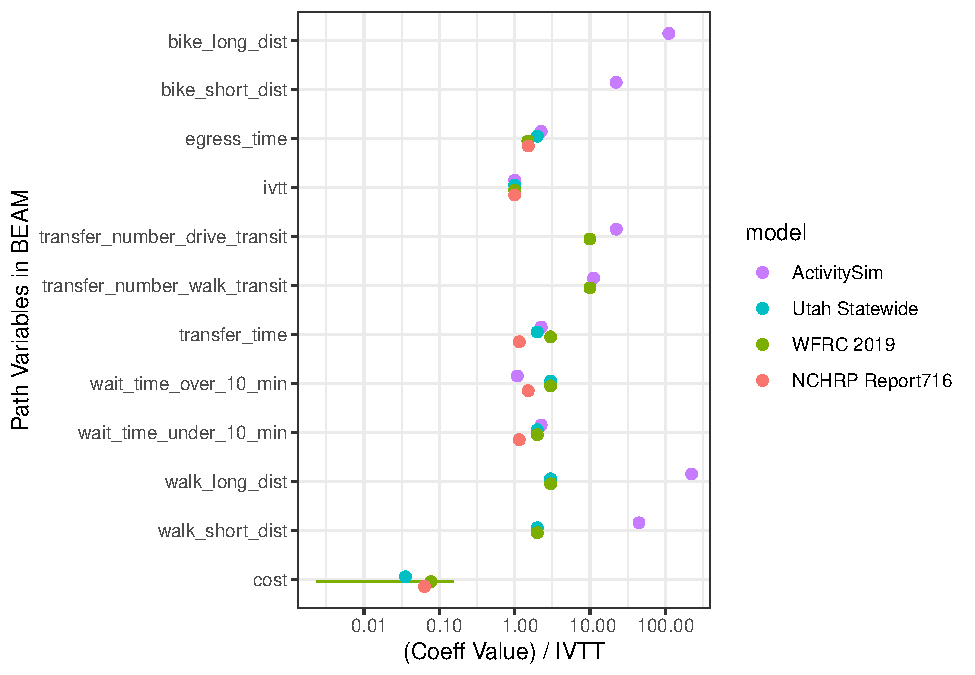
\includegraphics[width=400px]{thesis_files/figure-latex/hbw-1} 

}

\caption{Home-based work mode choice path coefficients model comparison.}\label{fig:hbw}
\end{figure}

Figure \ref{fig:hbs} shows the comparison of the path utility parameter values between all four models for home-based school trips. Similar to the home-based work analysis, for the egress time, ivtt, transfer time, and the wait times, ActivitySim seems to use a very similar coefficient value as the other three models. Again, the largest discrepancy exists with short and long walking distances. Since this is simply a difference between how walk distance is modeled, the discrepancy is ignored. In addition, the other three models did not have information on number of transfers. As a result, there is no comparison done with number of transfers. ActivitySim's path coefficient values do not require calibration for the home-based school parameters.

\begin{figure}

{\centering 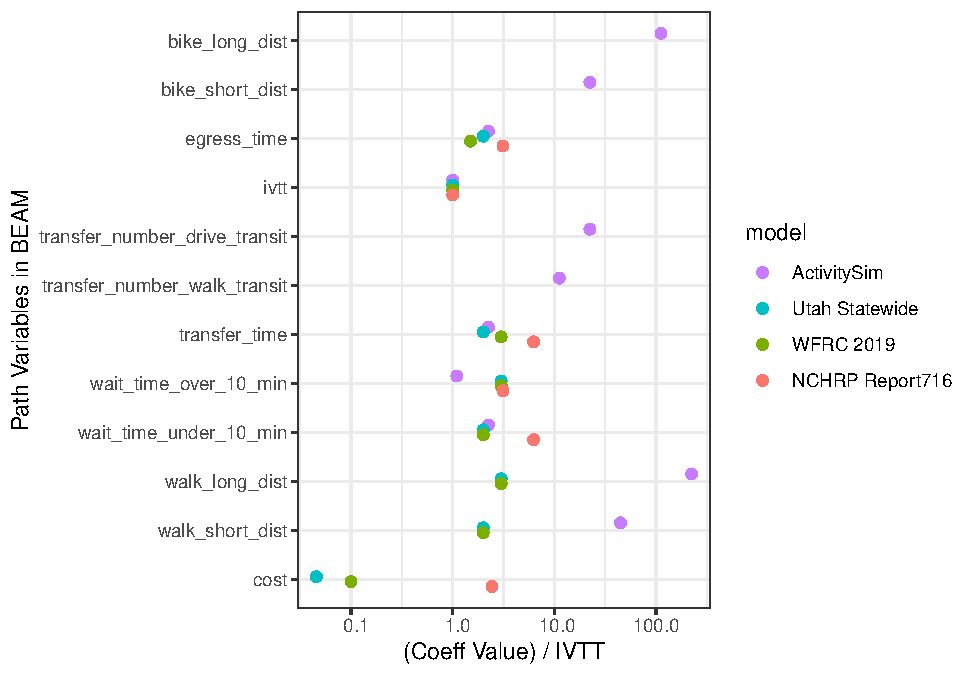
\includegraphics[width=400px]{thesis_files/figure-latex/hbs-1} 

}

\caption{Home-based school mode choice path coefficients model comparison.}\label{fig:hbs}
\end{figure}

Lastly, Figure \ref{fig:hbo} shows the comparison of path utility parameter values between all four models for home-based other trips. Again, besides for walk distance all variables seem to be similar between all four models. An interesting point is that for models other than ActivitySim, the cost coefficient varies greatly. Fortunately, ActivitySim bases the cost coefficient on each individual's value of time so this is not a concern. Overall, for all purpose types the coefficients used by ActivitySim are similar enough to other models that exist, and therefore do not require calibration. The ActivitySim alternative specific constants do, however, require calibration (See Section \ref{clib}).

\begin{figure}

{\centering 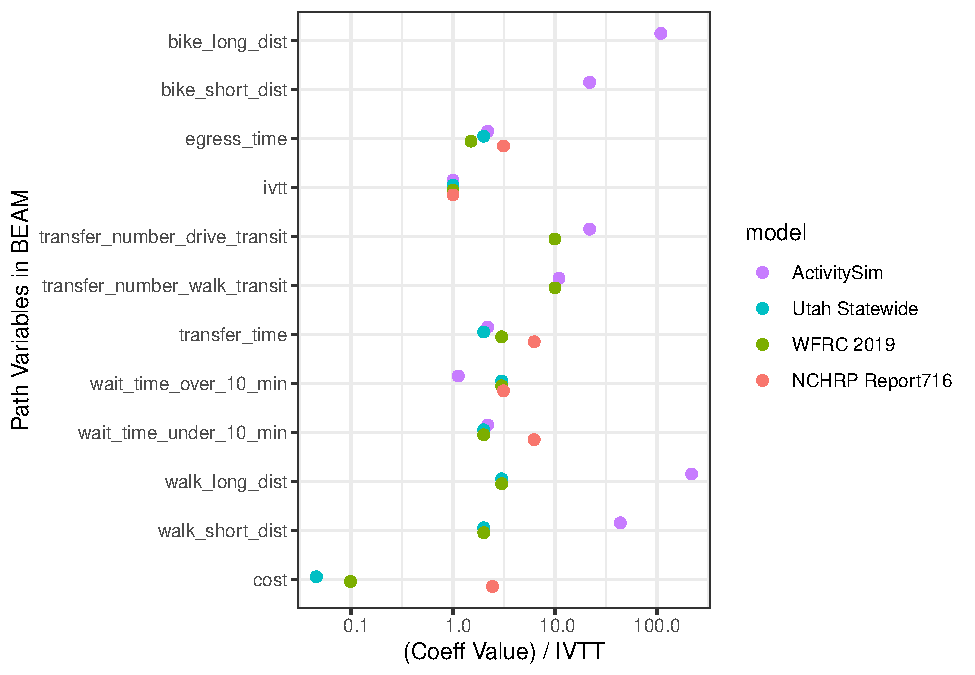
\includegraphics[width=400px]{thesis_files/figure-latex/hbo-1} 

}

\caption{Home-based other mode choice path coefficients model comparison.}\label{fig:hbo}
\end{figure}

\hypertarget{clib}{%
\subsection{Mode Choice Calibration}\label{clib}}

\hypertarget{summary}{%
\section{Summary}\label{summary}}

\hypertarget{results}{%
\chapter{Results}\label{results}}

\hypertarget{total-modal-distribution}{%
\section{Total Modal Distribution}\label{total-modal-distribution}}

\hypertarget{path-person-and-location-analysis}{%
\section{Path, Person, and Location Analysis}\label{path-person-and-location-analysis}}

\hypertarget{subtour-trip-analysis}{%
\section{Subtour Trip Analysis}\label{subtour-trip-analysis}}

\hypertarget{discussion}{%
\chapter{Discussion}\label{discussion}}

\hypertarget{conclusions}{%
\chapter{Conclusions}\label{conclusions}}

\cleardoublepage
    \bookmarksetupnext{level=part}
    \phantomsection
    \addcontentsline{toc}{chapter}{References}
    \begin{centering}
    REFERENCES\\
    \vskip 1 \baselineskip
    \end{centering}

\hypertarget{refs}{}
\begin{CSLReferences}{1}{0}
\leavevmode\vadjust pre{\hypertarget{ref-asim}{}}%
ActivitySim. 2021. \emph{ActivitySim: An Open Platform for Activity-Based Travel Modeling} (version 0.9.9.1). \url{https://github.com/ActivitySim/activitysim.}

\leavevmode\vadjust pre{\hypertarget{ref-rsg21}{}}%
{``ActivitySim: An Advanced Activity-Based Travel Demand Model Built by and for Users.''} 2021. \emph{RSG}. \url{https://rsginc.com/activitysim-white-paper/\#advanced-activity-based-travel-demand-model}.

\leavevmode\vadjust pre{\hypertarget{ref-agrc}{}}%
AGRC. 2021. \emph{Automated Geographic Reference Center}. \url{https://gis.utah.gov/}.

\leavevmode\vadjust pre{\hypertarget{ref-arentze00}{}}%
Arentze, Theo, and Harry Timmermans. 2000. \emph{Albatross: A Learning Based Transportation Oriented Simulation System}. Citeseer.

\leavevmode\vadjust pre{\hypertarget{ref-ax08}{}}%
Axhausen, K, M Balmer, and F Ciari. 2008. {``A New Mode Choice Model for a Multi-Agent Transport Simulation.''} In \emph{8th Swiss Transport Research Conference. ETH, Eidgen{ö}ssische Technische Hochschule}.

\leavevmode\vadjust pre{\hypertarget{ref-barth20}{}}%
Barth, Matthew, Peng Hao, Guoyuan Wu, Shams Tanvir, Chao Wang, Jeff Gonder, Jacob Holden, Andrew Devall, and Bingrong Sun. 2020. {``Evaluating Energy Efficiency Opportunities from Connected and Automated Vehicle Deployments Coupled with Shared Mobility in California.''} University of California-Riverside.

\leavevmode\vadjust pre{\hypertarget{ref-beam}{}}%
BEAM. 2022. \emph{Behavior, Energy, Autonomy, and Mobility}. Lawrence Berkeley National Laboratory the UC Berkeley Institute for Transportation Studies. \url{https://beam.readthedocs.io/en/develop/users.html}.

\leavevmode\vadjust pre{\hypertarget{ref-ben02}{}}%
Ben-Akiva, Moshe, Daniel Mcfadden, Kenneth Train, Joan Walker, Chandra Bhat, Michel Bierlaire, Denis Bolduc, et al. 2002. {``Hybrid Choice Models: Progress and Challenges.''} \emph{Marketing Letters} 13 (3): 163--75. \url{https://doi.org/10.1023/a:1020254301302}.

\leavevmode\vadjust pre{\hypertarget{ref-ben02num2}{}}%
Ben-Akiva, Moshe, Joan Walker, Adriana T. Bernardino, Dinesh A. Gopinath, Taka Morikawa, and Amalia Polydoropoulou. 2002. {``Integration of Choice and Latent Variable Models.''} \emph{In Perpetual Motion}, 431--70. \url{https://doi.org/10.1016/b978-008044044-6/50022-x}.

\leavevmode\vadjust pre{\hypertarget{ref-bhat95}{}}%
Bhat, Chandra R. 1995. {``A Heteroscedastic Extreme Value Model of Intercity Travel Mode Choice.''} \emph{Transportation Research Part B: Methodological} 29 (6): 471--83.

\leavevmode\vadjust pre{\hypertarget{ref-bhat99}{}}%
Bhat, Chandra R, and Frank S Koppelman. 1999. {``Activity-Based Modeling of Travel Demand.''} In \emph{Handbook of Transportation Science}, 35--61. Springer.

\leavevmode\vadjust pre{\hypertarget{ref-bowman01}{}}%
Bowman, J. L, and M. E Ben-Akiva. 2001. {``Activity-Based Disaggregate Travel Demand Model System with Activity Schedules.''} \emph{Transportation Research Part A: Policy and Practice} 35 (1): 1--28. \url{https://doi.org/10.1016/s0965-8564(99)00043-9}.

\leavevmode\vadjust pre{\hypertarget{ref-bowman06}{}}%
Bowman, John L., Mark A. Bradley, and John Gibbs. 2006. {``The Sacramento Activity-Based Travel Demand Model: Estimation and Validation Results.''} \emph{In European Transport Conference.}

\leavevmode\vadjust pre{\hypertarget{ref-bowman99}{}}%
Bowman, John L, Mark Bradley, Yoram Shiftan, T Keith Lawton, and Moshe Ben-Akiva. 1999. {``Demonstration of an Activity-Based Model for Portland.''} In \emph{World Transport Research: Selected Proceedings of the 8th World Conference on Transport ResearchWorld Conference on Transport Research Society}. Volume 3.

\leavevmode\vadjust pre{\hypertarget{ref-nchrp}{}}%
Cambridge Systematics, Inc., Inc. Vanasse Hangen Brustlin, Gallop Corporation, Chandra R. Bhat, LLC Shapiro Transportation Consulting, and PLLC Martin/Alexiou/Bryson. 2012. {``Travel Demand Forecasting: Parameters and Techniques.''} In \emph{NCHRP Report 716}, 55--60. Transportation Research Board.

\leavevmode\vadjust pre{\hypertarget{ref-r5}{}}%
Conveyal. 2022. \emph{R5: Rapid Realistic Routing on Real-World and Reimagined Networks}. \url{https://github.com/conveyal/r5}.

\leavevmode\vadjust pre{\hypertarget{ref-zarwi17}{}}%
El Zarwi, Feras, Akshay Vij, and Joan L Walker. 2017. {``A Discrete Choice Framework for Modeling and Forecasting the Adoption and Diffusion of New Transportation Services.''} \emph{Transportation Research Part C: Emerging Technologies} 79: 207--23.

\leavevmode\vadjust pre{\hypertarget{ref-eluru10}{}}%
Eluru, Naveen, Abdul Pinjari, Ram Pendyala, and Chandra Bhat. 2010. {``An Econometric Multi-Dimensional Choice Model of Activity-Travel Behavior.''} \emph{Transportation Letters} 2 (4): 217--30. \url{https://doi.org/10.3328/tl.2010.02.04.217-230}.

\leavevmode\vadjust pre{\hypertarget{ref-gali08}{}}%
Gali, Emmanuel, Stephan Eidenbenz, Sue Mniszewski, Leticia Cuellar, and Christof Teuscher. 2008. {``ActivitySim: Large-Scale Agent Based Activity Generation for Infrastructure Simulation,''} January. \url{https://www.osti.gov/biblio/960770}.

\leavevmode\vadjust pre{\hypertarget{ref-bhat20}{}}%
Goulias, Konstadinos G., Adam Wilkinson Davis, and Chandra R. Bhat. 2020. {``Chapter 5 - Consumer Choice Modeling: The Promises and the Cautions.''} In \emph{Mapping the Travel Behavior Genome}, 63--80. Elsevier.

\leavevmode\vadjust pre{\hypertarget{ref-hasnine21}{}}%
Hasnine, Md Sami, and Khandker Nurul Habib. 2021. {``Tour-Based Mode Choice Modelling as the Core of an Activity-Based Travel Demand Modelling Framework: A Review of State-of-the-Art.''} \emph{Transport Reviews} 41 (1): 5--26. \url{https://doi.org/10.1080/01441647.2020.1780648}.

\leavevmode\vadjust pre{\hypertarget{ref-horl18}{}}%
Hörl, Sebastian, Milos Balac, and Kay W Axhausen. 2018. {``A First Look at Bridging Discrete Choice Modeling and Agent-Based Microsimulation in MATSim.''} \emph{Procedia Computer Science} 130: 900--907.

\leavevmode\vadjust pre{\hypertarget{ref-horl19}{}}%
Hörl, Sebastian, Miloš Balać, and Kay W Axhausen. 2019. {``Pairing Discrete Mode Choice Models and Agent-Based Transport Simulation with MATSim.''} In \emph{2019 TRB Annual Meeting Online}, 19--02409. Transportation Research Board.

\leavevmode\vadjust pre{\hypertarget{ref-nate}{}}%
Lant, Nathan John. 2021. {``Estimation and Simulation of Daily Activity Patterns for Individuals Using Wheelchairs.''} PhD thesis, Brigham Young University.

\leavevmode\vadjust pre{\hypertarget{ref-manski2001}{}}%
Manski, Charles F. 2001. {``Daniel McFadden and the Econometric Analysis of Discrete Choice.''} \emph{The Scandinavian Journal of Economics} 103 (2): 217--29.

\leavevmode\vadjust pre{\hypertarget{ref-mcfadden1973}{}}%
McFadden, Daniel et al. 1973. {``Conditional Logit Analysis of Qualitative Choice Behavior.''}

\leavevmode\vadjust pre{\hypertarget{ref-mcfadden86}{}}%
McFadden, Daniel. 1986. {``The Choice Theory Approach to Market Research.''} \emph{Marketing Science} 5 (4): 275--97.

\leavevmode\vadjust pre{\hypertarget{ref-mcnally2000four}{}}%
McNally, Michael G. 2000. {``The Four Step Model.''} In \emph{Handbook of Transport Modelling}. Emerald Group Publishing Limited.

\leavevmode\vadjust pre{\hypertarget{ref-miller05}{}}%
Miller, Eric J., Matthew J. Roorda, and Juan Antonio Carrasco. 2005. {``A Tour-Based Model of Travel Mode Choice.''} \emph{Transportation} 32 (4): 399--422. \url{https://doi.org/10.1007/s11116-004-7962-3}.

\leavevmode\vadjust pre{\hypertarget{ref-mtc12}{}}%
MTC. 2012. \emph{Travel Model Development: Calibration and Validation Technical Report}. Metropolitan Transportation Commission with Parsons Brinckerhoff, Inc.

\leavevmode\vadjust pre{\hypertarget{ref-habib17}{}}%
Nurul Habib, Khandker. 2017. {``A Comprehensive Utility-Based System of Activity-Travel Scheduling Options Modelling (Custom) for Worker's Daily Activity Scheduling Processes.''} \emph{Transportmetrica A: Transport Science} 14 (4): 292--315. \url{https://doi.org/10.1080/23249935.2017.1385656}.

\leavevmode\vadjust pre{\hypertarget{ref-ortuzar94}{}}%
Ortuzar, J.de D., and L. G.Willumsen. 1994. Wiley.

\leavevmode\vadjust pre{\hypertarget{ref-paulssen14}{}}%
Paulssen, Marcel, Dirk Temme, Akshay Vij, and Joan L. Walker. 2014. {``Values, Attitudes and Travel Behavior: A Hierarchical Latent Variable Mixed Logit Model of Travel Mode Choice.''} \emph{Transportation} 41 (4): 873--88. \url{https://doi.org/10.1007/s11116-013-9504-3}.

\leavevmode\vadjust pre{\hypertarget{ref-pendyala05}{}}%
Pendyala, Ram M., Ryuichi Kitamura, Akira Kikuchi, Toshiyuki Yamamoto, and Satoshi Fujii. 2005. {``Florida Activity Mobility Simulator.''} \emph{Transportation Research Record: Journal of the Transportation Research Board} 1921 (1): 123--30. \url{https://doi.org/10.1177/0361198105192100114}.

\leavevmode\vadjust pre{\hypertarget{ref-pendyala97}{}}%
Pendyala, Ram M, Ryuichi Kitamura, Cynthia Chen, and Eric I Pas. 1997. {``An Activity-Based Microsimulation Analysis of Transportation Control Measures.''} \emph{Transport Policy} 4 (3): 183--92.

\leavevmode\vadjust pre{\hypertarget{ref-pinjari07}{}}%
Pinjari, Abdul Rawoof, Ram M. Pendyala, Chandra R. Bhat, and Paul A. Waddell. 2007. {``Modeling Residential Sorting Effects to Understand the Impact of the Built Environment on Commute Mode Choice.''} \emph{Transportation} 34 (5): 557--73. \url{https://doi.org/10.1007/s11116-007-9127-7}.

\leavevmode\vadjust pre{\hypertarget{ref-popsim}{}}%
PopulationSim. 2021. \emph{An Open Platform for Population Synthesis} (version 0.5). \url{https://activitysim.github.io/populationsim/}.

\leavevmode\vadjust pre{\hypertarget{ref-saleem18}{}}%
Saleem, Mohammad, Oskar Blom Västberg, and Anders Karlström. 2018. {``An Activity Based Demand Model for Large Scale Simulations.''} \emph{Procedia Computer Science} 130: 920--25.

\leavevmode\vadjust pre{\hypertarget{ref-utahstate}{}}%
UDOT. 2021. \emph{Utah State Travel Demand Model}. Utah Department of Transportation.

\leavevmode\vadjust pre{\hypertarget{ref-gtfs}{}}%
UTA. 2021. {``OpenMobilityData - GTFS.''} Utah Transit Authority. \url{https://transitfeeds.com/p/utah-transportation-authority/59}.

\leavevmode\vadjust pre{\hypertarget{ref-vij13}{}}%
Vij, Akshay, André Carrel, and Joan L. Walker. 2013. {``Incorporating the Influence of Latent Modal Preferences on Travel Mode Choice Behavior.''} \emph{Transportation Research Part A: Policy and Practice} 54: 164--78. \url{https://doi.org/10.1016/j.tra.2013.07.008}.

\leavevmode\vadjust pre{\hypertarget{ref-vovsha17}{}}%
Vovsha, P., J. E. Hicks, G. Vyas, V. Livshits, K. Jeon, R. Anderson, and G. Giaimo. 2017. {``Combinatorial Tour Mode Choice.''} In \emph{Presented at He 96th Annual Meeting of Transportation Research Board}.

\leavevmode\vadjust pre{\hypertarget{ref-horni16}{}}%
W Axhausen, Kay, Andreas Horni, and Kai Nagel. 2016. \emph{The Multi-Agent Transport Simulation MATSim}. Ubiquity Press.

\leavevmode\vadjust pre{\hypertarget{ref-wfrc}{}}%
WFRC. 2019. \emph{Wasatch Front Travel Demand Model} (version v8.3.1). Wasatch Front Regional Council. \url{https://wfrc.org/programs/models-forecasting/}.

\end{CSLReferences}


% Index?

\end{document}
